\section{The test architectures}
\label{sec:tests}

On 6--7 November 2026 every feature of the application was tried by hand on real machines (the checklist is \file{TEST\_APP.md} in the
repository). For that, eighteen small projects were built, \emph{TEST 1} to \emph{TEST 19} (there is no TEST 18: that number was a project
saved and deleted to test \ui{Delete}). Each is a working example of one kind of network, and most were trained on a Kaggle GPU or an
AWS EC2 g4dn.xlarge. This section shows each design as it looks on the Design screen, explains why it is built that way, and lists every
block with its output shape and parameter count. The counts are the application's own; they are the same numbers PyTorch reports
(checked for every block kind by the automatic tests).

Most of these networks are deliberately tiny: they test that a feature works end to end (data, shapes, training, results), not how good
a network can be. Projects 2--10, 14 and 15 use \emph{generated} data (patterns drawn by a script, so the right answer is known);
1, 11, 12, 13, 16, 17 and 19 use real data (EuroSAT, CIFAR-10, and Sentinel-1/2 exported from Google Earth Engine).

\paragraph{How the parameters are counted.} The counts follow from a few rules (Section~\ref{sec:blocks} has every block):
\begin{itemize}[nosep]
  \item Conv2D: $k_h \cdot k_w \cdot C_{in} \cdot C_{out}$ weights $+\,C_{out}$ biases. A 3$\times$3 convolution from 16 to 32 channels:
        $3\cdot 3\cdot 16\cdot 32 + 32 = 4\,640$. Conv3D adds the date kernel: $k_t\cdot k_h\cdot k_w\cdot C_{in}\cdot C_{out} + C_{out}$.
  \item Dense: $n_{in}\cdot n_{out} + n_{out}$. BatchNorm, LayerNorm: $2C$ (scale and shift); RMSNorm: $C$.
  \item Self-attention with dimension $d$: four $d\times d$ projections with biases, $4d^2 + 4d$.
  \item LSTM with $h$ units on $n$ inputs: $4(nh + h^2 + 2h)$ per direction; GRU: $3(nh + h^2 + 2h)$.
  \item LoRA of rank $r$ on a $n_{in}\times n_{out}$ layer adds $r(n_{in} + n_{out})$ trainable weights; the original weights are
        \emph{frozen} (kept, not trained). \emph{Frozen} blocks keep their weights fixed too; they still count in the total.
  \item Pooling, activations, Add, Concat, Subtract, Flatten, Dropout and \emph{Shared weights} have no parameters of their own (a shared
        block uses the weights of the block it copies, so they are counted once).
\end{itemize}
The screenshots were taken from copies of the projects in a neutral settings folder; the block ids in the tables (\texttt{t2},
\texttt{n10} \ldots) are the ids in the project's \file{model.json} and on the Text tab.


{\small
\begin{longtable}{@{}lp{4.4cm}lrrp{3.6cm}@{}}
\toprule
\textbf{Test} & \textbf{What it tests} & \textbf{Input} & \textbf{Blocks} & \textbf{Parameters} & \textbf{Result}\\
\midrule\endhead
1 & every new block kind in one network, real EuroSAT-MS & $13\times64\times64$ & 22 & 170\,904 & 83.7\,\% (early exit 79.3\,\%), Kaggle T4\\
2 & numbers per image (regression), DistributedDataParallel & $2\times16\times16$ & 5 & 5\,010 & $R^2$ 0.998, Kaggle T4$\times$2\\
3 & extra outputs (multi-task): a class, two numbers, a second class & $2\times16\times16$ & 9 & 6\,198 & class 100\,\%, $R^2$ 0.987, second class 97.5\,\%\\
4 & several classes per image, S2 + S1 early fusion & $5\times24\times24$ & 6 & 10\,819 & micro-F1 1.0\\
5 & mid fusion, Sentinel-2 at 32$\times$32 + Sentinel-1 at 16$\times$16 & $6\times32\times32$ & 9 & 7\,754 & 100\,\%\\
6 & shared weights (twin branch), $|a-b|$, custom loss & $4\times24\times24$ & 9 & 2\,658 & 100\,\%\\
7 & dates as a sequence: Conv1D, GRU, LSTM & $2\times6\times16\times16$ & 7 & 6\,610 & 100\,\%\\
8 & segmentation of a time series: Conv3D + temporal attention & $2\times6\times16\times16$ & 6 & 10\,196 & 95.0\,\% pixels, mIoU 0.869\\
9 & boxes (CenterNet-style detection head) & $3\times64\times64$ & 9 & 26\,102 & mAP@0.5 0.951\\
10 & 200 : 20 images, class weights and focal loss & $2\times16\times16$ & 5 & 2\,658 & 100\,\% (weights 0.55 / 5.5)\\
11 & ImageNet weights + LoRA rank 4 on attention, real EuroSAT RGB & $3\times224\times224$ & 91 & 86\,027\,530 & 93.6\,\% training 228\,874 weights\\
12 & the same ViT, every weight trained & $3\times224\times224$ & 91 & 85\,806\,346 & 96.8\,\% training 85.8 M weights\\
13 & \file{everything.nnb}: all block kinds; recipe, 3 seeds, export & $3\times32\times32$ & 97 & 217\,396 & 50.95 $\pm$ 1.62\,\% (2 epochs, 3 seeds)\\
14 & the Text tab: \file{timeseries.nnb} pasted and edited & $4\times6\times32\times32$ & 18 & 27\,684 & built and checked (window test; not trained)\\
15 & a scene + label image cut into tiles, strip test split & $2\times16\times16$ & 4 & 2\,675 & 95.9\,\% pixels, mIoU 0.919\\
16 & Small CNN (CIFAR-10) demo on an EC2 g4dn.xlarge & $3\times32\times32$ & 29 & 551\,018 & 40.5\,\% (2 epochs), 79.5\,\% (10 epochs), Stop: 75.7\,\%\\
17 & 40 real S2 L1C + S1 exports, fused & $15\times64\times64$ & 7 & 23\,562 & data check passed (no training)\\
19 & the app's own GEE script: S2 + WorldCover, from a Drive link & $4\times64\times64$ & 5 & 10\,859 & 79.8\,\% pixels (built-up IoU 0.71, trees 0.67)\\
\bottomrule
\end{longtable}}

\subsection{TEST 1: a hybrid CNN + transformer on 13 Sentinel-2 bands}
\label{sec:test1}

TEST 1 puts nearly every block added in the architecture steps into one network and trains it on real data: EuroSAT-MS (Sentinel-2, all 13 bands, 64$\times$64 pixels, 10 land-cover classes), with focal loss and class weights.

\screenshot{figures/tests/test01.jpg}{TEST 1 on the Design screen: a convolutional front end, an early exit, then a transformer encoder with LoRA, SwiGLU and a mixture of experts.}{fig:test1}

\begin{figure}[htbp]\centering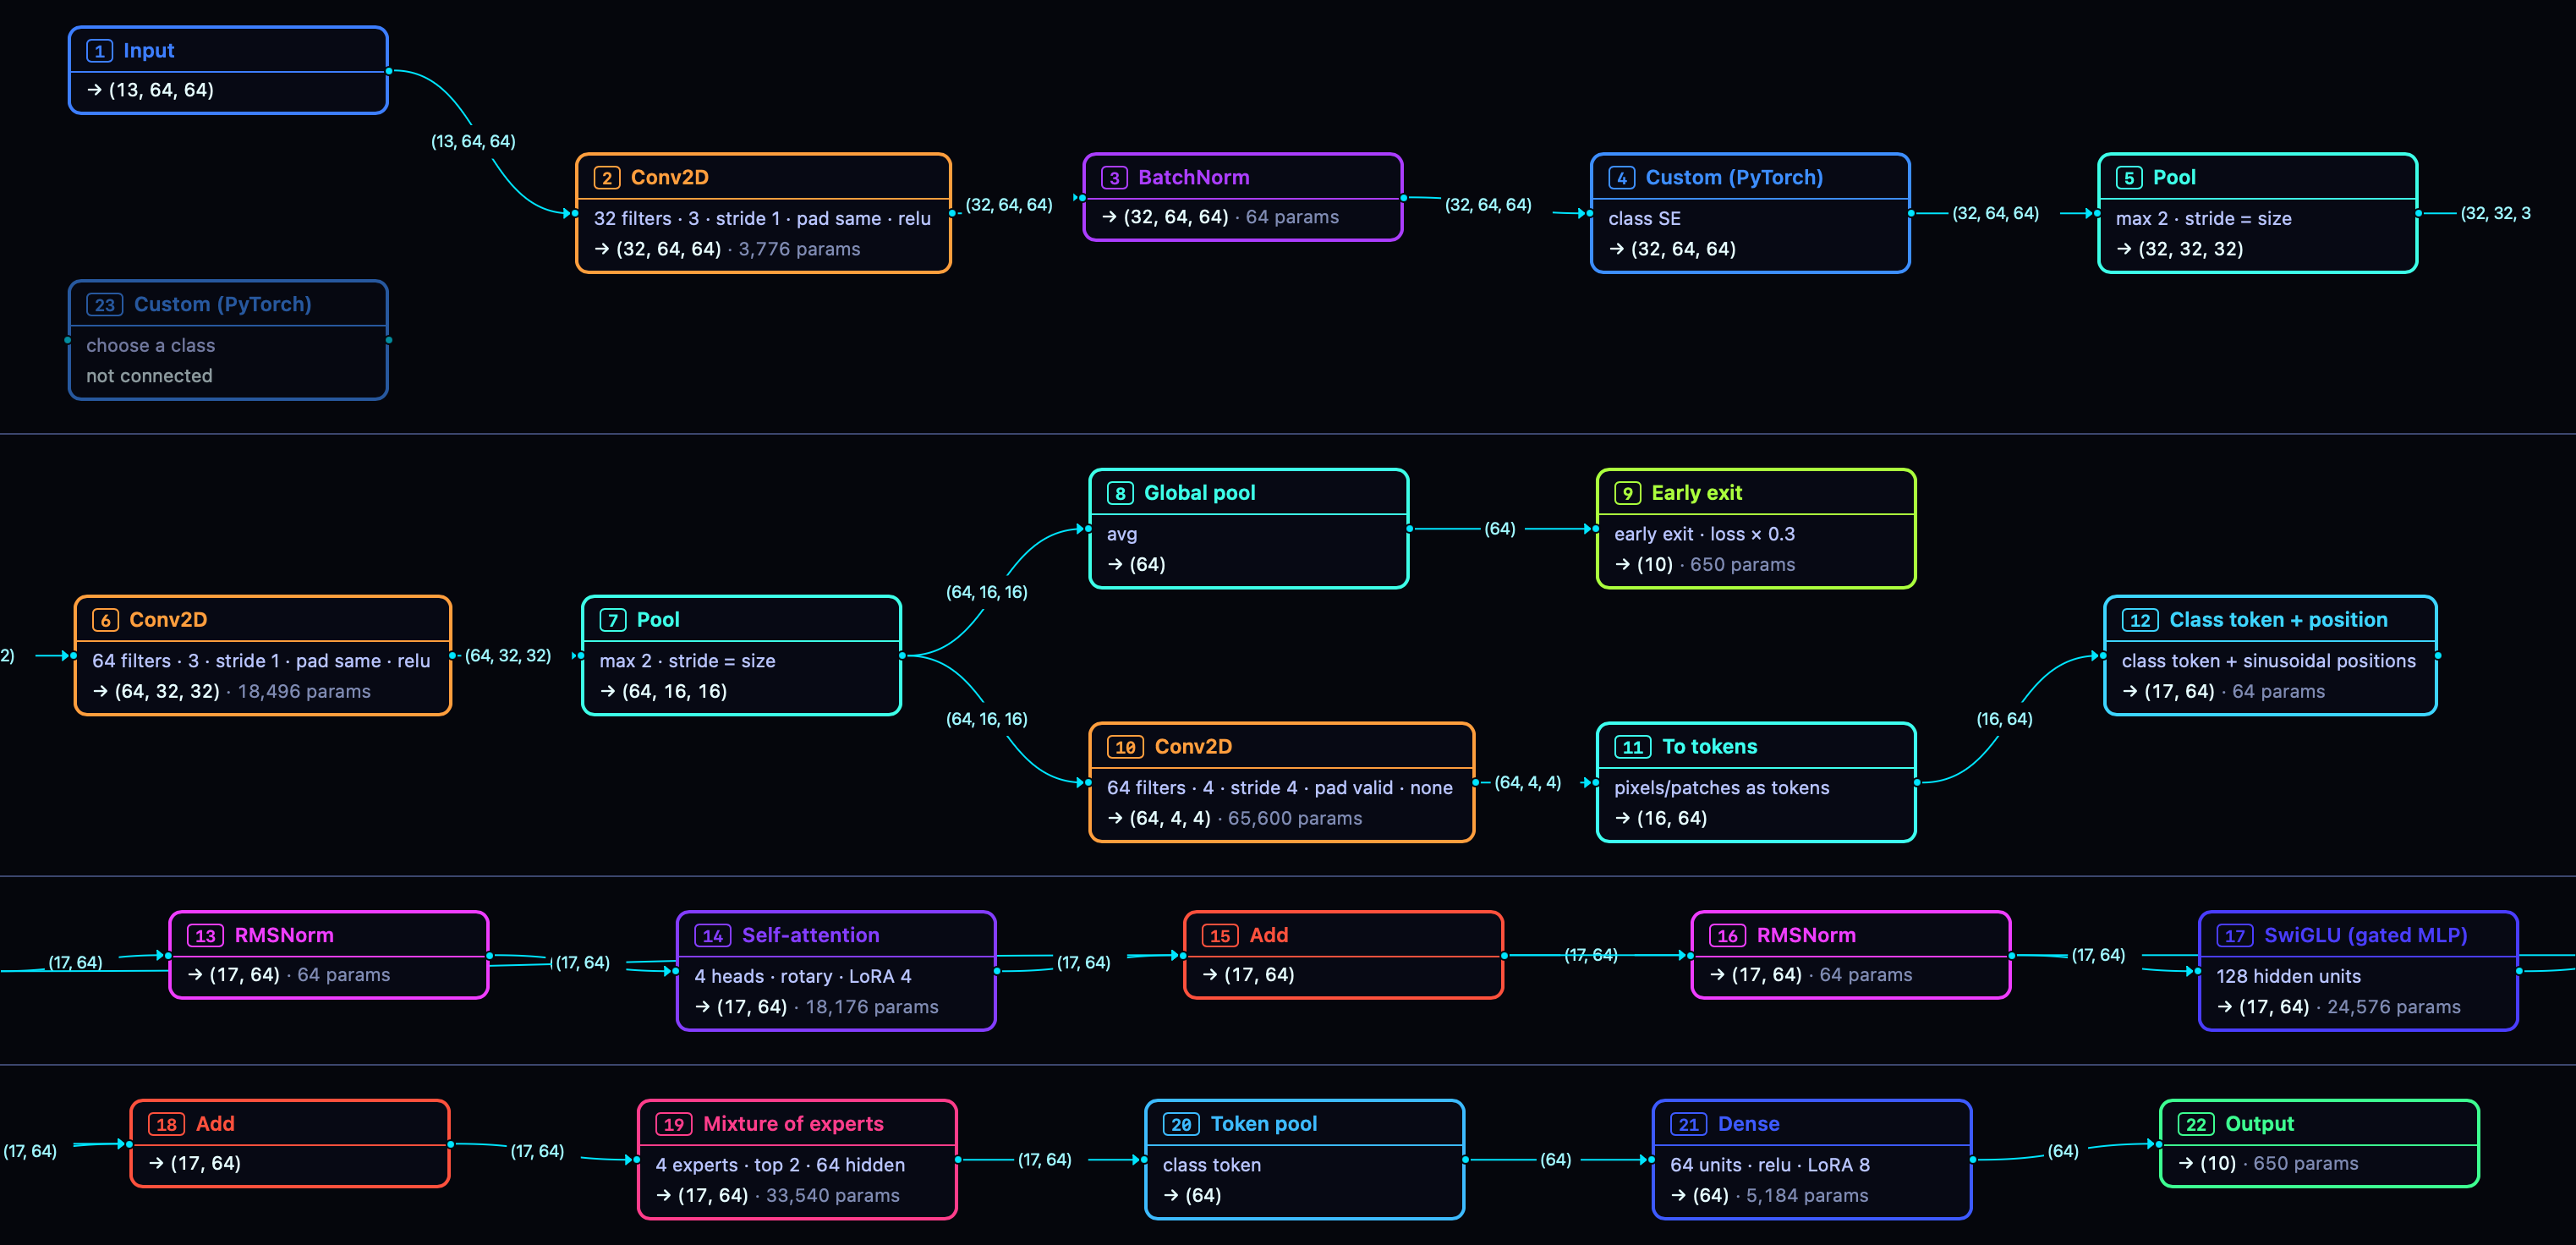
\includegraphics[width=\linewidth,height=0.55\textheight,keepaspectratio]{figures/tests/test01_arch.png}\caption{TEST 1 as a picture: \ui{Save as PNG} on the Design screen (or \ui{File} $\rightarrow$ \ui{Export Design as PNG}) draws the whole design at full size; long designs are split into rows here to fit the page.}\label{fig:test1arch}\end{figure}

The first convolution (32 filters, 3$\times$3 on 13 bands: $3\cdot 3\cdot 13\cdot 32+32=3\,776$) is \emph{frozen}, as if it came from an earlier model. A Custom block \texttt{SE} (squeeze-and-excitation, written in PyTorch on the Text tab) reweights the 32 channels. After two pooling steps the network branches: a global average pool feeds an \emph{early exit} (a small classifier, $64\cdot 10+10=650$, trained with loss weight 0.3) that can answer for easy images, while a 4$\times$4 convolution with stride 4 ($4\cdot4\cdot64\cdot64+64=65\,600$, the largest block) turns the 16$\times$16 map into 16 patches of 64 numbers. The transformer part adds a class token (sinusoidal positions have no weights, so only the token's 64 count), RMSNorm, self-attention with rotary positions and LoRA (base $4\cdot64^2+4\cdot64=16\,640$ frozen, LoRA rank 4 on q, k, v: $3\cdot4\cdot(64+64)=1\,536$), a SwiGLU feed-forward ($3\cdot 64\cdot 128=24\,576$, no biases) and a mixture of 4 experts (router $64\cdot4+4=260$, each expert two 64$\times$64 layers, $4\cdot 8\,320$, so 33\,540; each token uses its best 2). The classifier is a LoRA Dense (64 units, base 4\,160 frozen + rank 8: 1\,024) and the Output. Of 170\,904 parameters 24\,576 are frozen, so 146\,328 are trained; the SE block's 552 weights are counted on the training machine, not by the app.

{\small
\begin{longtable}{@{}lp{3.2cm}p{5.4cm}lr@{}}
\toprule
\textbf{Id} & \textbf{Block} & \textbf{Settings} & \textbf{Output} & \textbf{Parameters}\\
\midrule\endhead
t1 & Input & all bands & $13\times64\times64$ & 0\\
t2 & Conv2D & 32 filters, $3\times3$, same, relu, frozen & $32\times64\times64$ & 3\,776 (3\,776 frozen)\\
t3 & BatchNorm &  & $32\times64\times64$ & 64\\
t4 & Custom (PyTorch) & class SE & $32\times64\times64$ & 0\\
t5 & Pool & max 2$\times$2 & $32\times32\times32$ & 0\\
t6 & Conv2D & 64 filters, $3\times3$, same, relu & $64\times32\times32$ & 18\,496\\
t7 & Pool & max 2$\times$2 & $64\times16\times16$ & 0\\
t8 & Global pool & avg & $64$ & 0\\
t10 & Conv2D & 64 filters, $4\times4$, stride 4, pad valid & $64\times4\times4$ & 65\,600\\
t9 & Early exit & loss weight 0.3 & $10$ & 650\\
t11 & To tokens & patches & $16\times64$ & 0\\
t12 & Class token + positions & positions sinusoidal & $17\times64$ & 64\\
t13 & RMSNorm &  & $17\times64$ & 64\\
t14 & Self-attention & 4 heads, rotary, LoRA rank 4 & $17\times64$ & 18\,176 (16\,640 frozen)\\
t15 & Add &  & $17\times64$ & 0\\
t16 & RMSNorm &  & $17\times64$ & 64\\
t17 & SwiGLU & 128 hidden units & $17\times64$ & 24\,576\\
t18 & Add &  & $17\times64$ & 0\\
t19 & Mixture of experts & 4 experts, top 2, 64 units & $17\times64$ & 33\,540\\
t20 & Token pool & cls & $64$ & 0\\
t21 & Dense & 64 units, relu, LoRA rank 8 & $64$ & 5\,184 (4\,160 frozen)\\
t22 & Output & main output & $10$ & 650\\
\midrule
 & \textbf{Total} & & & \textbf{170\,904}\\
\bottomrule
\end{longtable}}

The design also holds one Custom block that is not connected (left from a test of the code editor); it has no shape and no parameters and is left out of the table.

\subsection{TEST 2: regression on two GPUs}
\label{sec:test2}

TEST 2 predicts two numbers per image (regression, Huber loss) instead of a class, and was trained on Kaggle's two T4 GPUs at once (the run split each batch between them).

\screenshot{figures/tests/test02.jpg}{TEST 2 on the Design screen: two convolutions, a global pool and an Output with one number per target.}{fig:test2}

\begin{figure}[htbp]\centering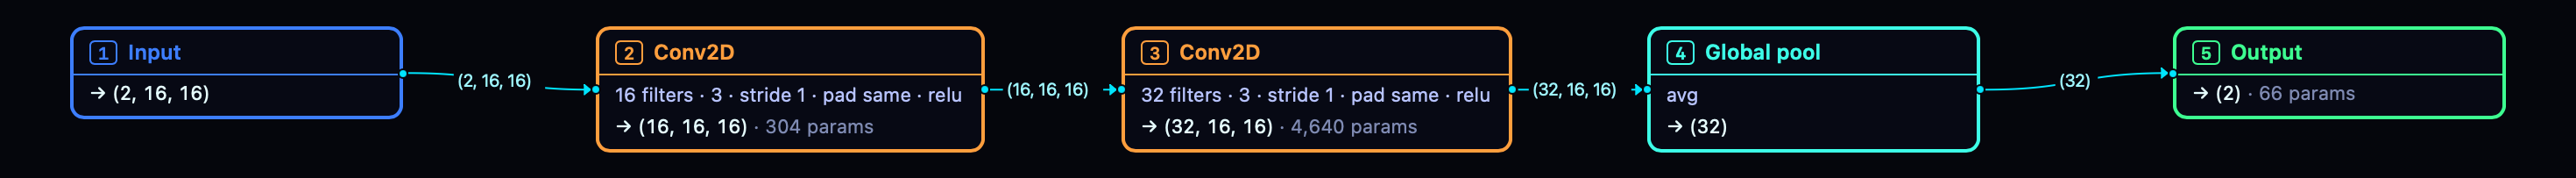
\includegraphics[width=\linewidth,height=0.55\textheight,keepaspectratio]{figures/tests/test02_arch.png}\caption{TEST 2 as a picture: \ui{Save as PNG} on the Design screen (or \ui{File} $\rightarrow$ \ui{Export Design as PNG}) draws the whole design at full size; long designs are split into rows here to fit the page.}\label{fig:test2arch}\end{figure}

The design is the smallest useful image regressor: a 3$\times$3 convolution from 2 bands to 16 channels ($3\cdot3\cdot2\cdot16+16=304$), one from 16 to 32 ($4\,640$), a global average pool that turns each 16$\times$16 map into one number, and an Output with one unit per target ($32\cdot 2+2=66$). The Output of a regression network has no softmax: its two numbers are the predictions (the app standardises the targets for training and converts back). This run also found a real bug: on two GPUs the training finished but a worker process never exited; the fix is in the application since.

{\small
\begin{longtable}{@{}lp{3.2cm}p{5.4cm}lr@{}}
\toprule
\textbf{Id} & \textbf{Block} & \textbf{Settings} & \textbf{Output} & \textbf{Parameters}\\
\midrule\endhead
t1 & Input & all bands & $2\times16\times16$ & 0\\
t2 & Conv2D & 16 filters, $3\times3$, same, relu & $16\times16\times16$ & 304\\
t3 & Conv2D & 32 filters, $3\times3$, same, relu & $32\times16\times16$ & 4\,640\\
t4 & Global pool & avg & $32$ & 0\\
t5 & Output & main output & $2$ & 66\\
\midrule
 & \textbf{Total} & & & \textbf{5\,010}\\
\bottomrule
\end{longtable}}

\subsection{TEST 3: one network, three outputs}
\label{sec:test3}

TEST 3 has one trunk and three heads: the main class (from the folder name), two numbers per image and a second class (both from a labels table). One loss is the weighted sum of the three.

\screenshot{figures/tests/test03.jpg}{TEST 3 on the Design screen: one trunk, three Output blocks: the main class, an extra output with two numbers and an extra output with a second class.}{fig:test3}

\begin{figure}[htbp]\centering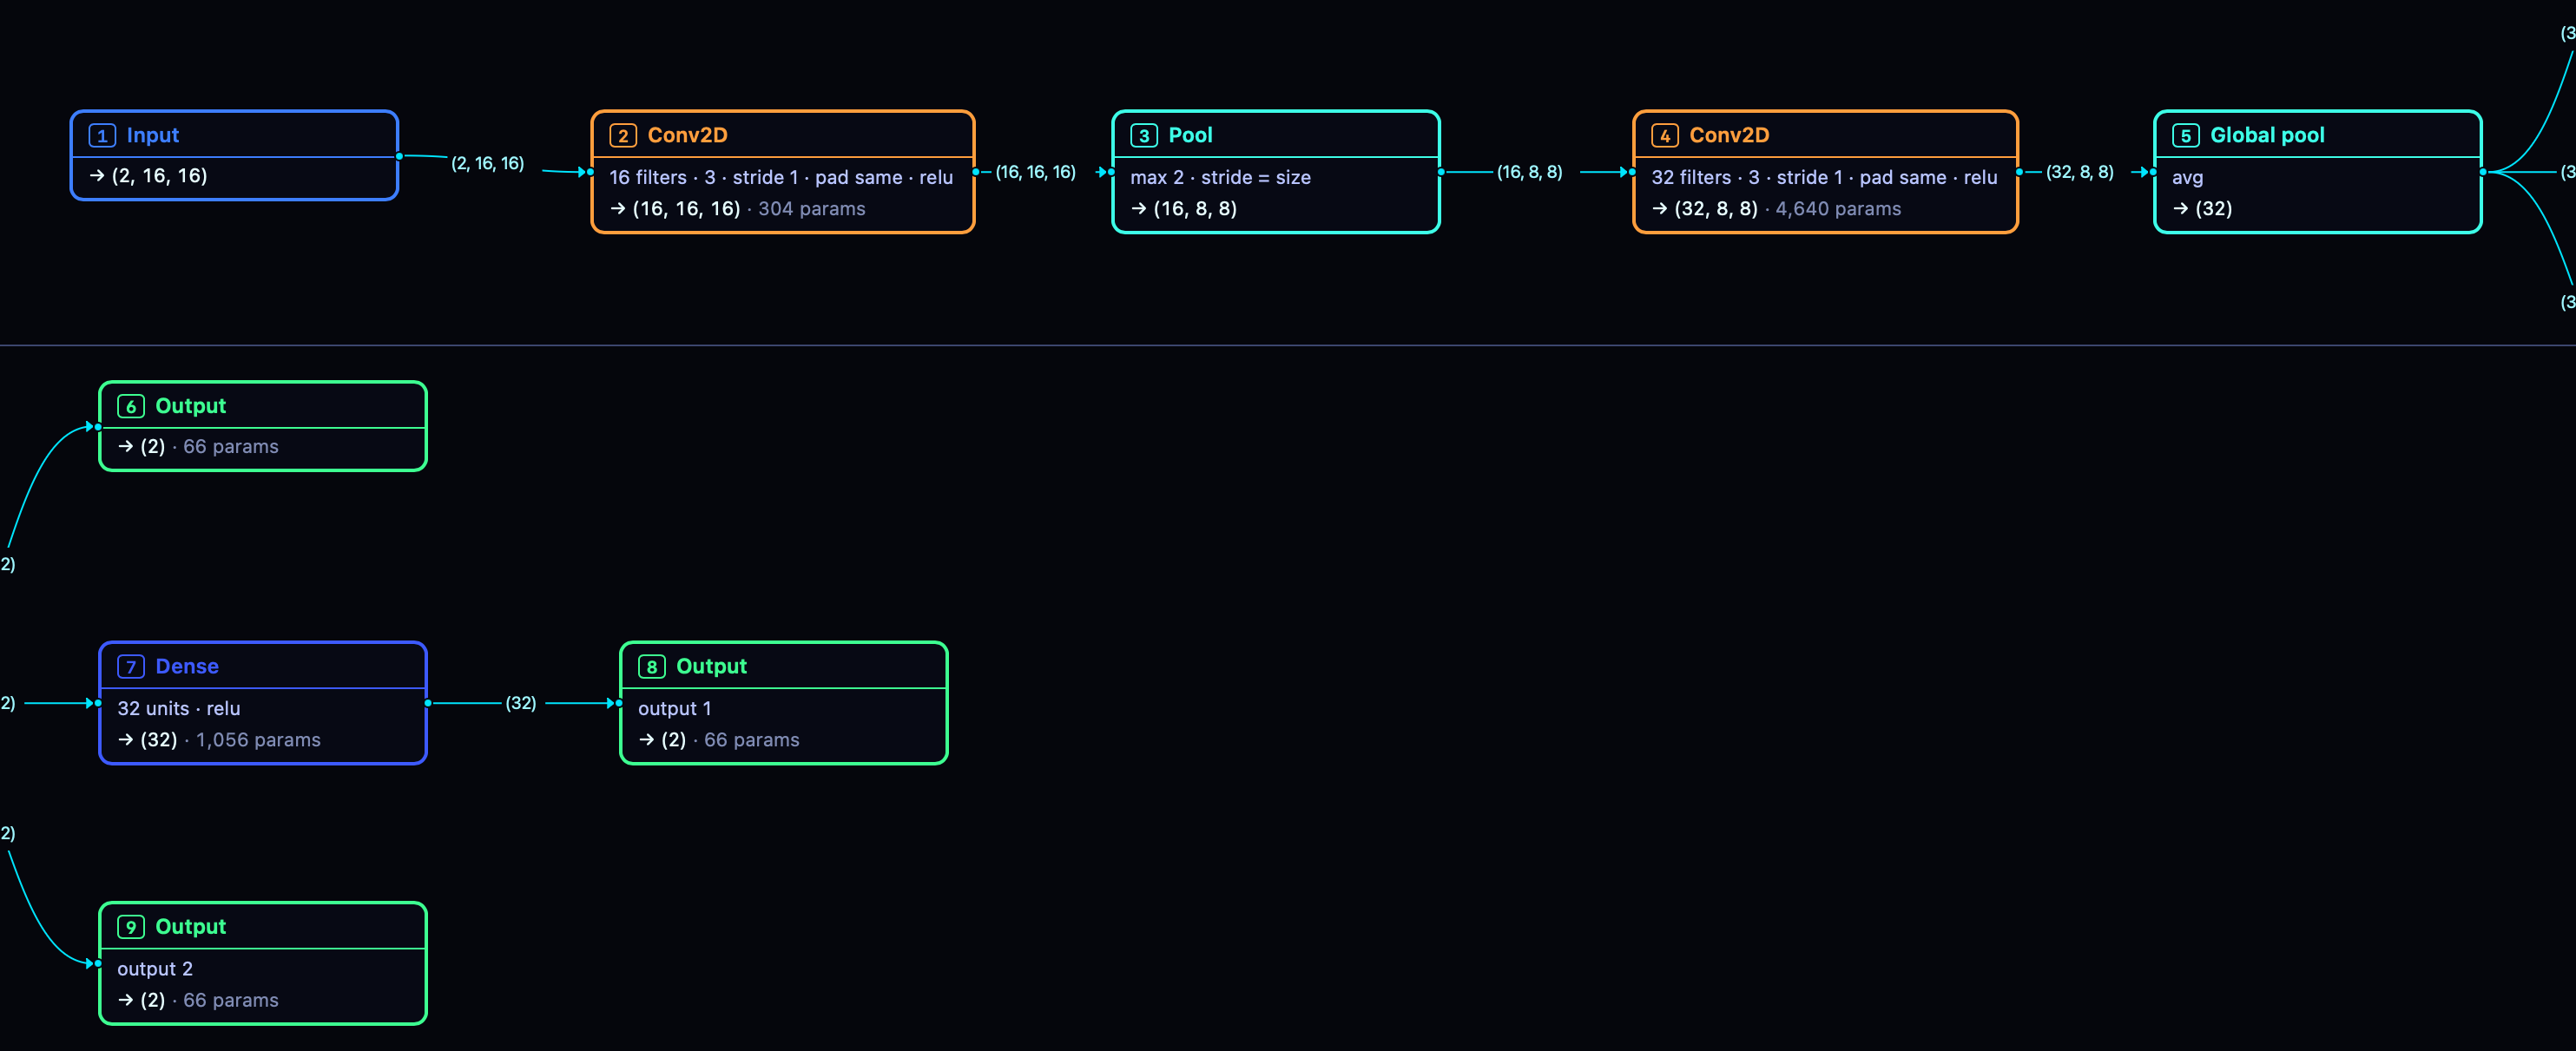
\includegraphics[width=\linewidth,height=0.55\textheight,keepaspectratio]{figures/tests/test03_arch.png}\caption{TEST 3 as a picture: \ui{Save as PNG} on the Design screen (or \ui{File} $\rightarrow$ \ui{Export Design as PNG}) draws the whole design at full size; long designs are split into rows here to fit the page.}\label{fig:test3arch}\end{figure}

The shared trunk (304 + 4\,640 parameters) learns features useful for all three tasks. The main Output and extra output 1 sit directly on the pooled 32 numbers ($32\cdot 2+2=66$ each); extra output 2 has its own Dense layer of 32 units first ($32\cdot32+32=1\,056$), the usual way to give one task a little more capacity. In the Output inspector, \ui{Output for} chooses which task an Output serves.

{\small
\begin{longtable}{@{}lp{3.2cm}p{5.4cm}lr@{}}
\toprule
\textbf{Id} & \textbf{Block} & \textbf{Settings} & \textbf{Output} & \textbf{Parameters}\\
\midrule\endhead
t1 & Input & all bands & $2\times16\times16$ & 0\\
t2 & Conv2D & 16 filters, $3\times3$, same, relu & $16\times16\times16$ & 304\\
t3 & Pool & max 2$\times$2 & $16\times8\times8$ & 0\\
t4 & Conv2D & 32 filters, $3\times3$, same, relu & $32\times8\times8$ & 4\,640\\
t5 & Global pool & avg & $32$ & 0\\
t6 & Output & main output & $2$ & 66\\
t7 & Dense & 32 units, relu & $32$ & 1\,056\\
t9 & Output & extra output 2 & $2$ & 66\\
t8 & Output & extra output 1 & $2$ & 66\\
\midrule
 & \textbf{Total} & & & \textbf{6\,198}\\
\bottomrule
\end{longtable}}

\subsection{TEST 4: multi-label with Sentinel-1 + Sentinel-2}
\label{sec:test4}

TEST 4 gives each image any number of classes at once (multi-label, a labels table) and stacks two sensors in one Input: three Sentinel-2 bands and the two Sentinel-1 radar bands (early fusion).

\screenshot{figures/tests/test04.jpg}{TEST 4 on the Design screen: five bands (three of Sentinel-2, two of Sentinel-1) enter one Input.}{fig:test4}

\begin{figure}[htbp]\centering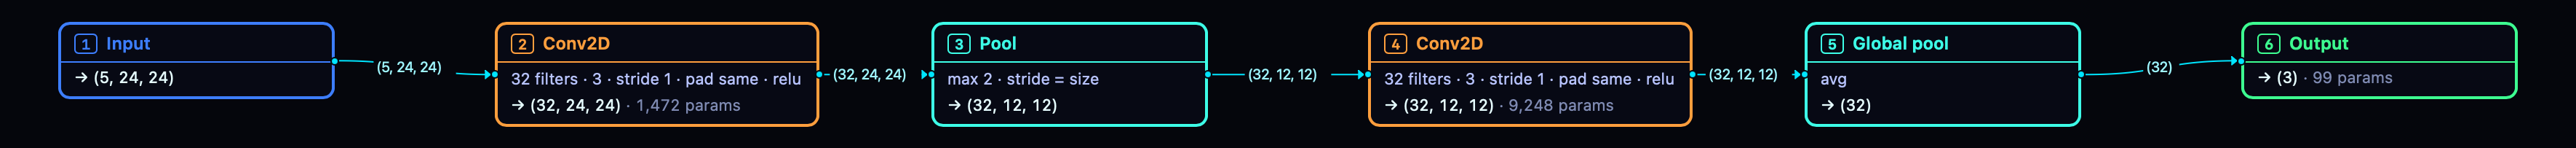
\includegraphics[width=\linewidth,height=0.55\textheight,keepaspectratio]{figures/tests/test04_arch.png}\caption{TEST 4 as a picture: \ui{Save as PNG} on the Design screen (or \ui{File} $\rightarrow$ \ui{Export Design as PNG}) draws the whole design at full size; long designs are split into rows here to fit the page.}\label{fig:test4arch}\end{figure}

With early fusion the first convolution simply sees 5 channels ($3\cdot3\cdot5\cdot32+32=1\,472$). The Output has one unit per class ($32\cdot 3+3=99$) and a sigmoid per unit instead of a softmax, so each class is a separate yes/no; the threshold per class can be tuned on the validation data.

{\small
\begin{longtable}{@{}lp{3.2cm}p{5.4cm}lr@{}}
\toprule
\textbf{Id} & \textbf{Block} & \textbf{Settings} & \textbf{Output} & \textbf{Parameters}\\
\midrule\endhead
t1 & Input & all bands & $5\times24\times24$ & 0\\
t2 & Conv2D & 32 filters, $3\times3$, same, relu & $32\times24\times24$ & 1\,472\\
t3 & Pool & max 2$\times$2 & $32\times12\times12$ & 0\\
t4 & Conv2D & 32 filters, $3\times3$, same, relu & $32\times12\times12$ & 9\,248\\
t5 & Global pool & avg & $32$ & 0\\
t6 & Output & main output & $3$ & 99\\
\midrule
 & \textbf{Total} & & & \textbf{10\,819}\\
\bottomrule
\end{longtable}}

\subsection{TEST 5: two sensors at their own sizes}
\label{sec:test5}

TEST 5 keeps each sensor at its own resolution (Sentinel-2 at 32$\times$32, Sentinel-1 at 16$\times$16), so nothing is invented by resizing, and joins them inside the network (mid fusion).

\screenshot{figures/tests/test05.jpg}{TEST 5 on the Design screen: two Inputs (band groups 1 and 2) with their own first layers, joined by Concat.}{fig:test5}

\begin{figure}[htbp]\centering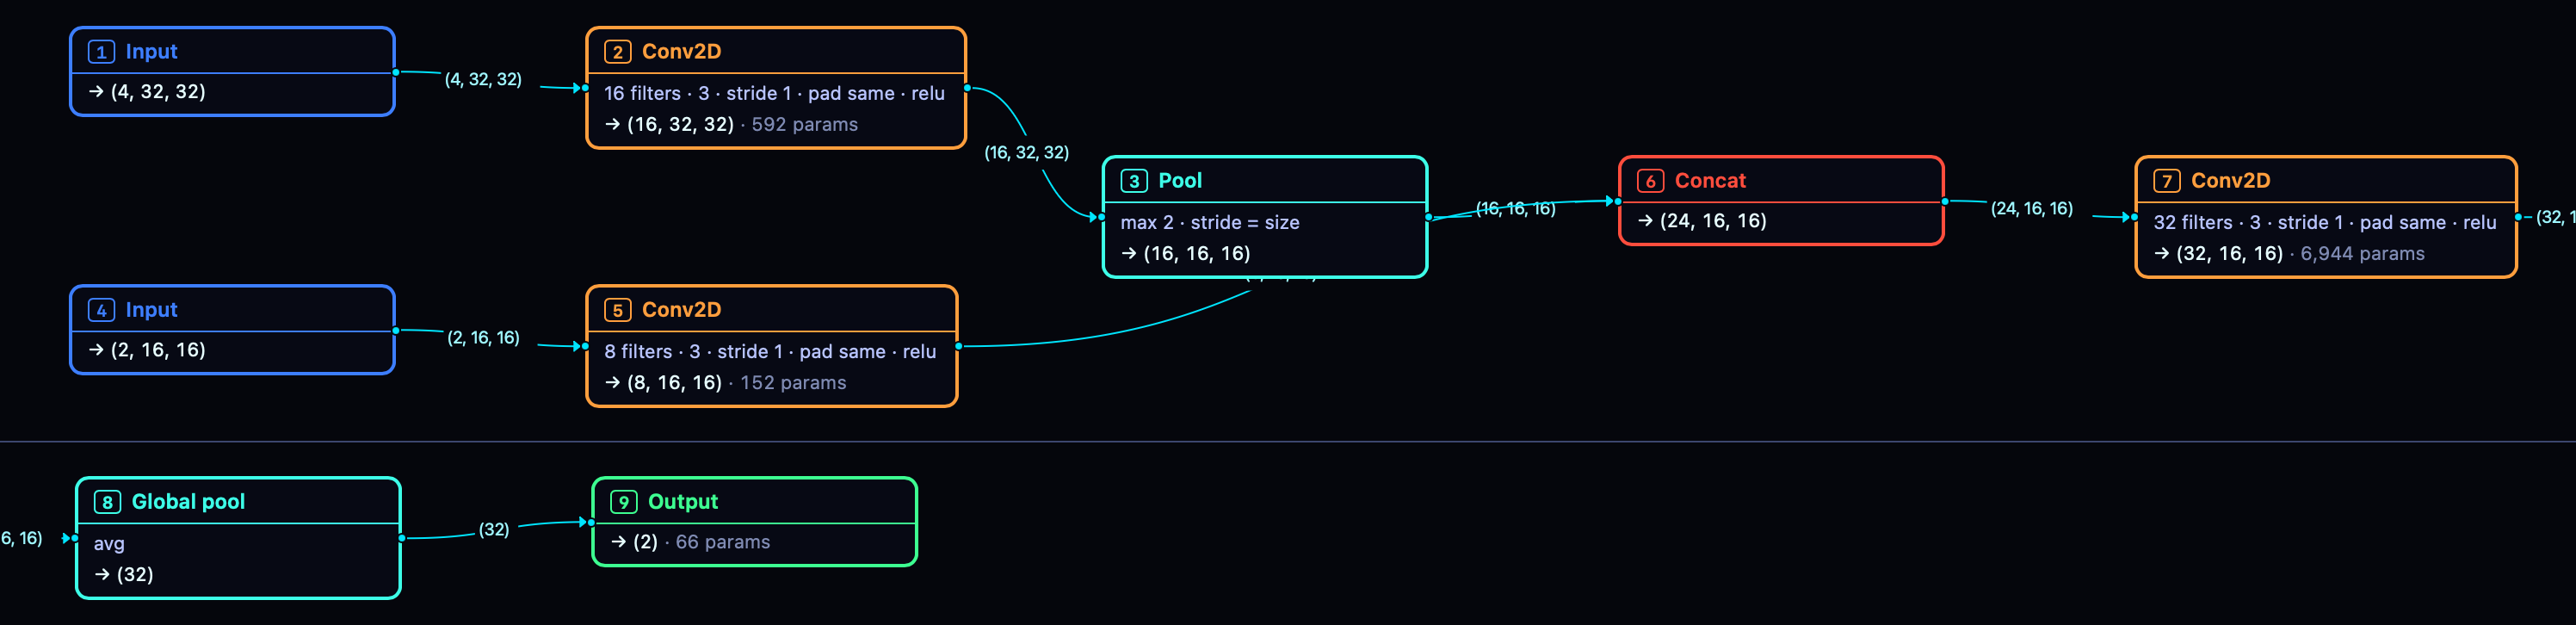
\includegraphics[width=\linewidth,height=0.55\textheight,keepaspectratio]{figures/tests/test05_arch.png}\caption{TEST 5 as a picture: \ui{Save as PNG} on the Design screen (or \ui{File} $\rightarrow$ \ui{Export Design as PNG}) draws the whole design at full size; long designs are split into rows here to fit the page.}\label{fig:test5arch}\end{figure}

Each Input takes one band group. The Sentinel-2 branch (4 bands, $3\cdot3\cdot4\cdot16+16=592$) is pooled to 16$\times$16 so that it meets the radar branch (2 bands, $3\cdot3\cdot2\cdot8+8=152$) at the same size; Concat stacks the 16 and 8 channels into 24, and a joint convolution ($3\cdot3\cdot24\cdot32+32=6\,944$) mixes the sensors. Concat itself has no parameters.

{\small
\begin{longtable}{@{}lp{3.2cm}p{5.4cm}lr@{}}
\toprule
\textbf{Id} & \textbf{Block} & \textbf{Settings} & \textbf{Output} & \textbf{Parameters}\\
\midrule\endhead
t1 & Input & band group 1 & $4\times32\times32$ & 0\\
t4 & Input & band group 2 & $2\times16\times16$ & 0\\
t2 & Conv2D & 16 filters, $3\times3$, same, relu & $16\times32\times32$ & 592\\
t5 & Conv2D & 8 filters, $3\times3$, same, relu & $8\times16\times16$ & 152\\
t3 & Pool & max 2$\times$2 & $16\times16\times16$ & 0\\
t6 & Concat &  & $24\times16\times16$ & 0\\
t7 & Conv2D & 32 filters, $3\times3$, same, relu & $32\times16\times16$ & 6\,944\\
t8 & Global pool & avg & $32$ & 0\\
t9 & Output & main output & $2$ & 66\\
\midrule
 & \textbf{Total} & & & \textbf{7\,754}\\
\bottomrule
\end{longtable}}

\subsection{TEST 6: a Siamese network for change}
\label{sec:test6}

TEST 6 decides whether something changed between two images of the same place (before and after), with a custom loss written in Python.

\screenshot{figures/tests/test06.jpg}{TEST 6 on the Design screen: two Inputs (before and after) through the same two convolutions, then the absolute difference.}{fig:test6}

\begin{figure}[htbp]\centering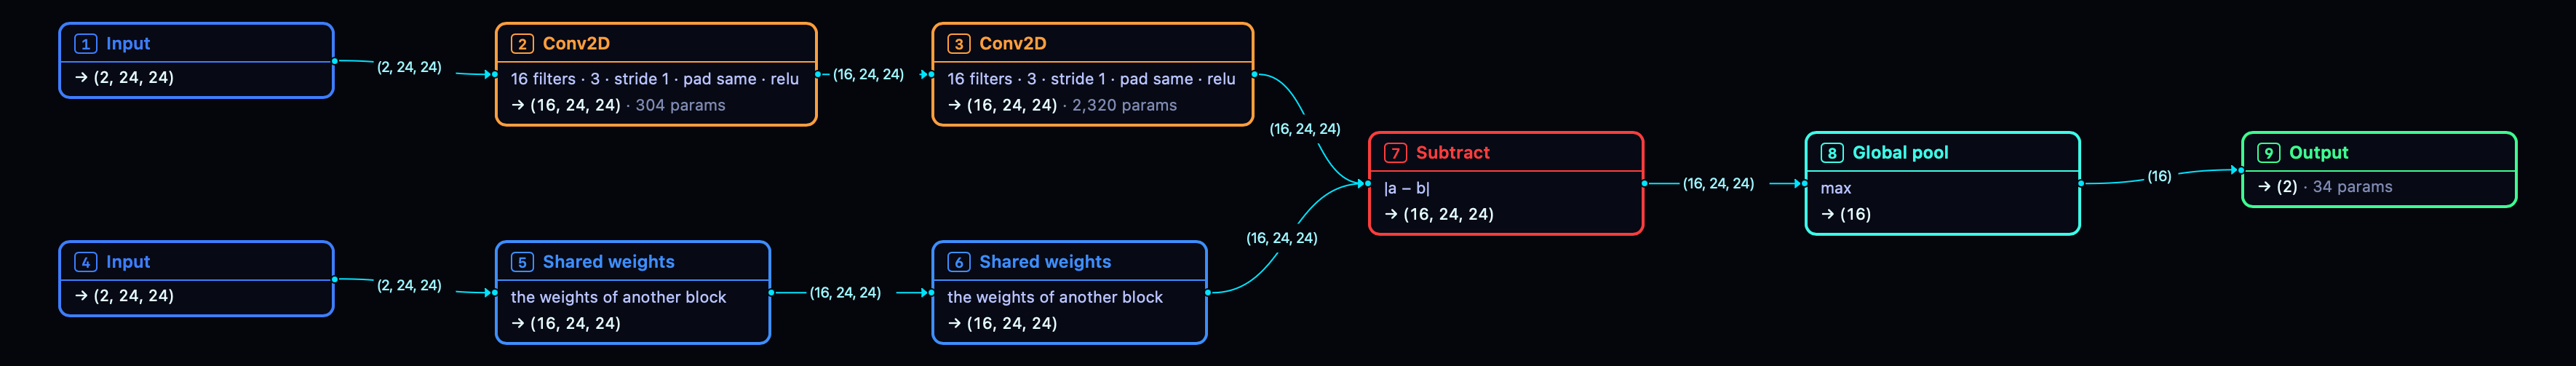
\includegraphics[width=\linewidth,height=0.55\textheight,keepaspectratio]{figures/tests/test06_arch.png}\caption{TEST 6 as a picture: \ui{Save as PNG} on the Design screen (or \ui{File} $\rightarrow$ \ui{Export Design as PNG}) draws the whole design at full size; long designs are split into rows here to fit the page.}\label{fig:test6arch}\end{figure}

Both images must be judged the same way, so the second branch does not have its own convolutions: its two blocks are \emph{Shared weights} copies of the first branch's (\ui{Twin branch} on the canvas). That is why the design has four convolution blocks but only two sets of weights ($304 + 2\,320$). Subtract with absolute value gives $|a-b|$ per pixel and channel, a global max pool keeps the strongest difference, and the Output says change / no change ($16\cdot2+2=34$). In total 2\,658 parameters, the same number PyTorch counts for the generated code.

{\small
\begin{longtable}{@{}lp{3.2cm}p{5.4cm}lr@{}}
\toprule
\textbf{Id} & \textbf{Block} & \textbf{Settings} & \textbf{Output} & \textbf{Parameters}\\
\midrule\endhead
t1 & Input & band group 1 & $2\times24\times24$ & 0\\
t4 & Input & band group 2 & $2\times24\times24$ & 0\\
t2 & Conv2D & 16 filters, $3\times3$, same, relu & $16\times24\times24$ & 304\\
t3 & Conv2D & 16 filters, $3\times3$, same, relu & $16\times24\times24$ & 2\,320\\
t5 & Shared weights & weights of block t2 & $16\times24\times24$ & 0\\
t6 & Shared weights & weights of block t3 & $16\times24\times24$ & 0\\
t7 & Subtract & $|a-b|$ & $16\times24\times24$ & 0\\
t8 & Global pool & max & $16$ & 0\\
t9 & Output & main output & $2$ & 34\\
\midrule
 & \textbf{Total} & & & \textbf{2\,658}\\
\bottomrule
\end{longtable}}

\subsection{TEST 7: a time series as a sequence}
\label{sec:test7}

TEST 7 classifies a stack of six dates (2 bands, 16$\times$16 pixels each) by how the image changes over time.

\screenshot{figures/tests/test07.jpg}{TEST 7 on the Design screen: To sequence, then a 1-D convolution, a bidirectional GRU and an LSTM over the six dates.}{fig:test7}

\begin{figure}[htbp]\centering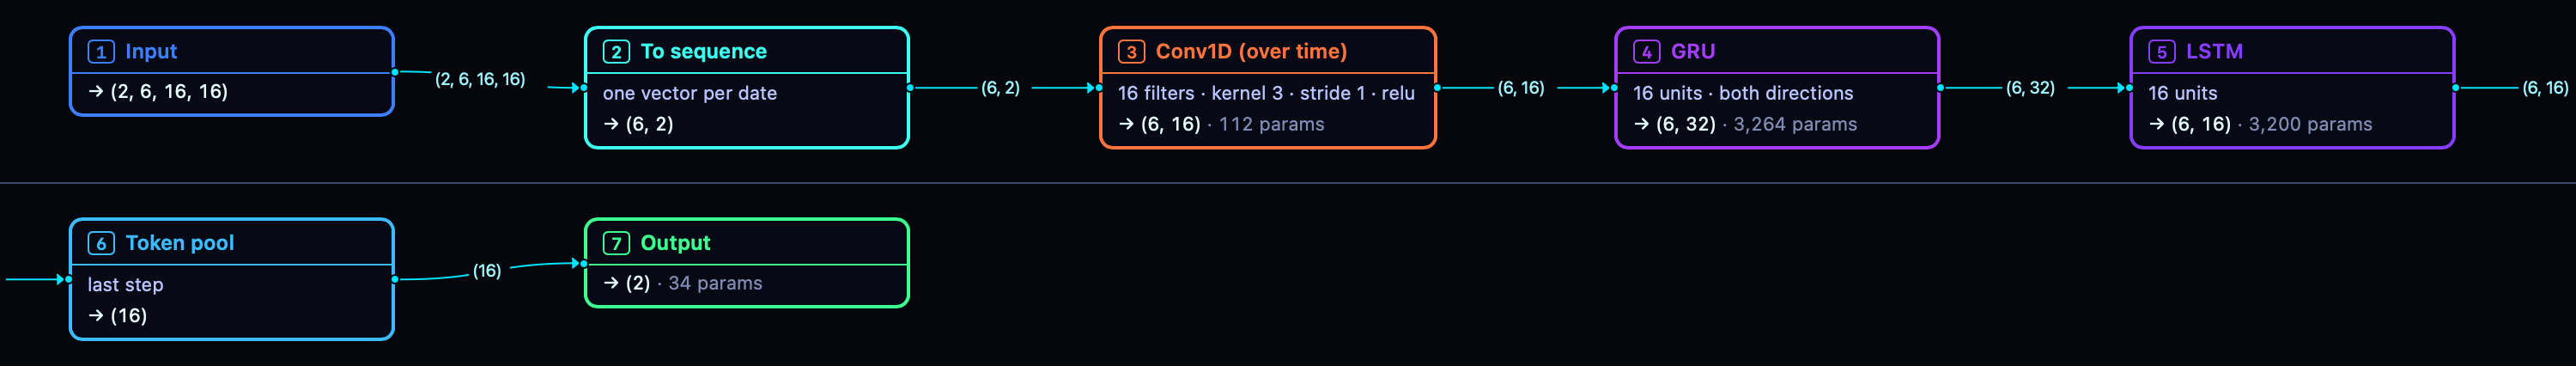
\includegraphics[width=\linewidth,height=0.55\textheight,keepaspectratio]{figures/tests/test07_arch.png}\caption{TEST 7 as a picture: \ui{Save as PNG} on the Design screen (or \ui{File} $\rightarrow$ \ui{Export Design as PNG}) draws the whole design at full size; long designs are split into rows here to fit the page.}\label{fig:test7arch}\end{figure}

\emph{To sequence} averages each date's pixels, so the six dates become a sequence of six 2-number vectors. A Conv1D looks at three neighbouring dates at a time ($3\cdot2\cdot16+16=112$). A bidirectional GRU (16 units each way: $2\cdot3\cdot(16\cdot16+16\cdot16+2\cdot16)=3\,264$) reads the sequence forwards and backwards, an LSTM of 16 units on its 32 numbers ($4\cdot(32\cdot16+16\cdot16+2\cdot16)=3\,200$) reads it again, and \emph{Token pool: last} keeps the state after the last date.

{\small
\begin{longtable}{@{}lp{3.2cm}p{5.4cm}lr@{}}
\toprule
\textbf{Id} & \textbf{Block} & \textbf{Settings} & \textbf{Output} & \textbf{Parameters}\\
\midrule\endhead
t1 & Input & all bands & $2\times6\times16\times16$ & 0\\
t2 & To sequence &  & $6\times2$ & 0\\
t3 & Conv1D & 16 filters, kernel 3, relu & $6\times16$ & 112\\
t4 & GRU & 16 units, both directions & $6\times32$ & 3\,264\\
t5 & LSTM & 16 units & $6\times16$ & 3\,200\\
t6 & Token pool & last & $16$ & 0\\
t7 & Output & main output & $2$ & 34\\
\midrule
 & \textbf{Total} & & & \textbf{6\,610}\\
\bottomrule
\end{longtable}}

\subsection{TEST 8: a crop map from a time series}
\label{sec:test8}

TEST 8 labels every pixel (segmentation) from a stack of six dates: the kind of network used for crop-type maps.

\screenshot{figures/tests/test08.jpg}{TEST 8 on the Design screen: two Conv3D layers over dates and pixels, temporal attention, a Conv2D and the Segmentation output.}{fig:test8}

\begin{figure}[htbp]\centering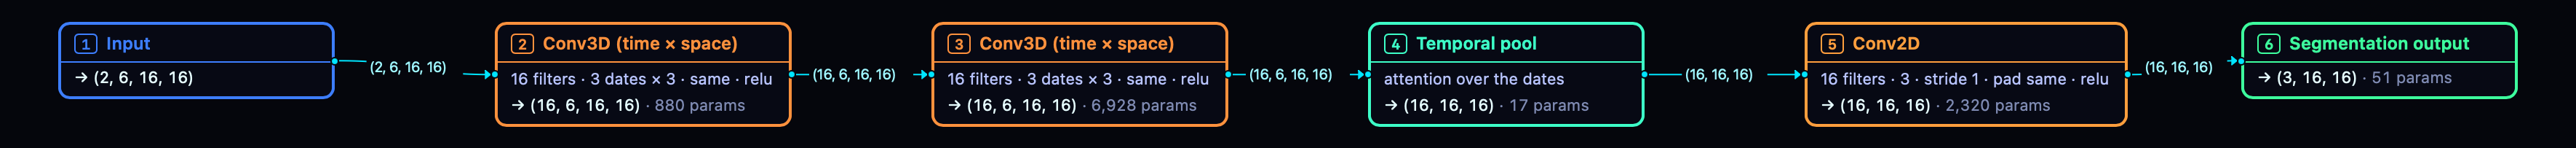
\includegraphics[width=\linewidth,height=0.55\textheight,keepaspectratio]{figures/tests/test08_arch.png}\caption{TEST 8 as a picture: \ui{Save as PNG} on the Design screen (or \ui{File} $\rightarrow$ \ui{Export Design as PNG}) draws the whole design at full size; long designs are split into rows here to fit the page.}\label{fig:test8arch}\end{figure}

A Conv3D kernel spans 3 dates and 3$\times$3 pixels ($3\cdot3\cdot3\cdot2\cdot16+16=880$, then $3\cdot3\cdot3\cdot16\cdot16+16=6\,928$), so it sees how each neighbourhood changes. \emph{Temporal pool: attention} then weighs the six dates per pixel and sums them into one image (17 weights: one score per channel plus a bias). A 2-D convolution refines it, and the Segmentation output gives 3 class scores per pixel (a 1$\times$1 convolution, $16\cdot3+3=51$).

{\small
\begin{longtable}{@{}lp{3.2cm}p{5.4cm}lr@{}}
\toprule
\textbf{Id} & \textbf{Block} & \textbf{Settings} & \textbf{Output} & \textbf{Parameters}\\
\midrule\endhead
t1 & Input & all bands & $2\times6\times16\times16$ & 0\\
t2 & Conv3D & 16 filters, $3\times3$ over 3 dates, relu & $16\times6\times16\times16$ & 880\\
t3 & Conv3D & 16 filters, $3\times3$ over 3 dates, relu & $16\times6\times16\times16$ & 6\,928\\
t4 & Temporal pool & attention & $16\times16\times16$ & 17\\
t5 & Conv2D & 16 filters, $3\times3$, same, relu & $16\times16\times16$ & 2\,320\\
t6 & Segmentation output &  & $3\times16\times16$ & 51\\
\midrule
 & \textbf{Total} & & & \textbf{10\,196}\\
\bottomrule
\end{longtable}}

\subsection{TEST 9: object detection}
\label{sec:test9}

TEST 9 finds objects and draws boxes (two classes, squares and discs, in generated images with YOLO-format box labels).

\screenshot{figures/tests/test09.jpg}{TEST 9 on the Design screen: four convolutions with two poolings, then the Detection output on a quarter-size map.}{fig:test9}

\begin{figure}[htbp]\centering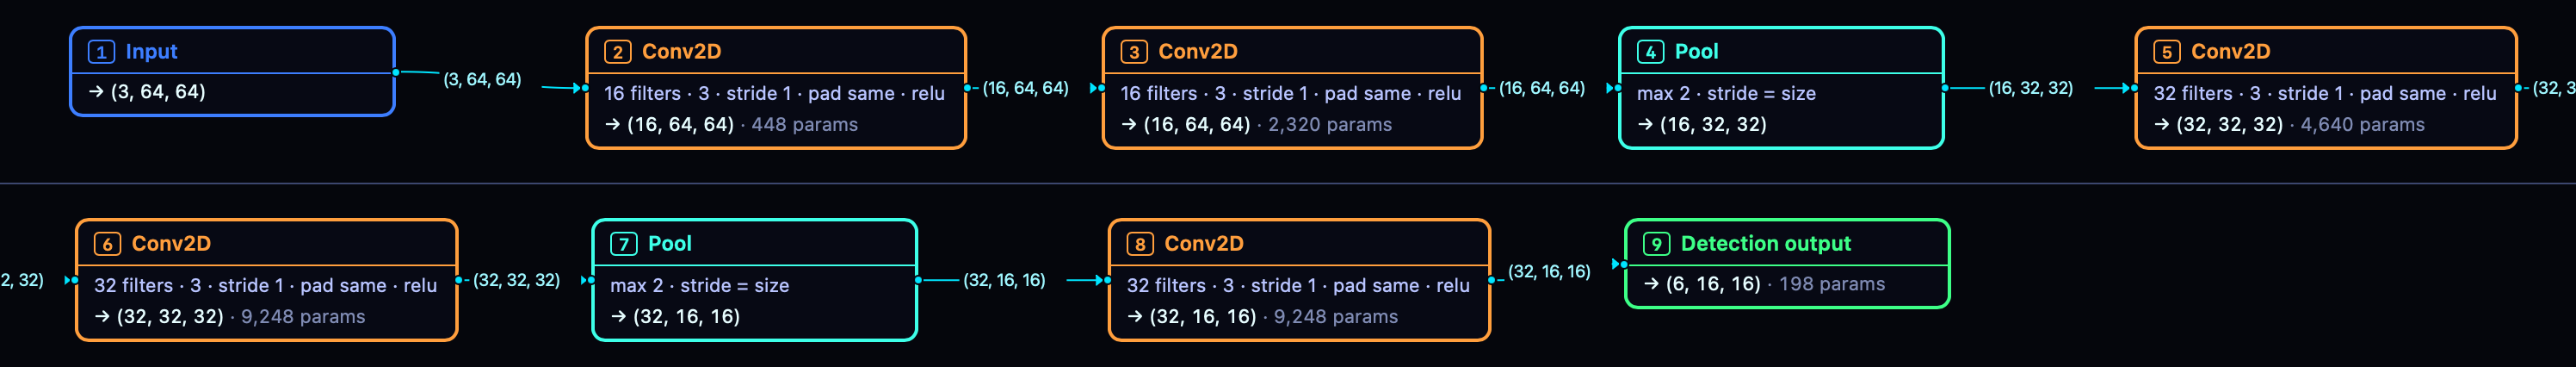
\includegraphics[width=\linewidth,height=0.55\textheight,keepaspectratio]{figures/tests/test09_arch.png}\caption{TEST 9 as a picture: \ui{Save as PNG} on the Design screen (or \ui{File} $\rightarrow$ \ui{Export Design as PNG}) draws the whole design at full size; long designs are split into rows here to fit the page.}\label{fig:test9arch}\end{figure}

The backbone halves the 64$\times$64 image twice (16 $\rightarrow$ 32 channels, 448 to 9\,248 parameters per convolution). The Detection output is a 1$\times$1 convolution that gives, for every cell of the 16$\times$16 map, one score per class (\emph{is an object centred here?}) and four numbers (box width, height and the centre's offset): $32\cdot(2+4)+(2+4)=198$. Each cell is 4$\times$4 pixels of the input; the strongest peaks become the boxes.

{\small
\begin{longtable}{@{}lp{3.2cm}p{5.4cm}lr@{}}
\toprule
\textbf{Id} & \textbf{Block} & \textbf{Settings} & \textbf{Output} & \textbf{Parameters}\\
\midrule\endhead
t1 & Input & all bands & $3\times64\times64$ & 0\\
t2 & Conv2D & 16 filters, $3\times3$, same, relu & $16\times64\times64$ & 448\\
t3 & Conv2D & 16 filters, $3\times3$, same, relu & $16\times64\times64$ & 2\,320\\
t4 & Pool & max 2$\times$2 & $16\times32\times32$ & 0\\
t5 & Conv2D & 32 filters, $3\times3$, same, relu & $32\times32\times32$ & 4\,640\\
t6 & Conv2D & 32 filters, $3\times3$, same, relu & $32\times32\times32$ & 9\,248\\
t7 & Pool & max 2$\times$2 & $32\times16\times16$ & 0\\
t8 & Conv2D & 32 filters, $3\times3$, same, relu & $32\times16\times16$ & 9\,248\\
t9 & Detection output &  & $6\times16\times16$ & 198\\
\midrule
 & \textbf{Total} & & & \textbf{26\,102}\\
\bottomrule
\end{longtable}}

\subsection{TEST 10: unbalanced classes}
\label{sec:test10}

TEST 10 trains on 200 images of one class and 20 of the other, where a careless network learns to always answer the common class.

\screenshot{figures/tests/test10.jpg}{TEST 10 on the Design screen: a two-convolution classifier.}{fig:test10}

\begin{figure}[htbp]\centering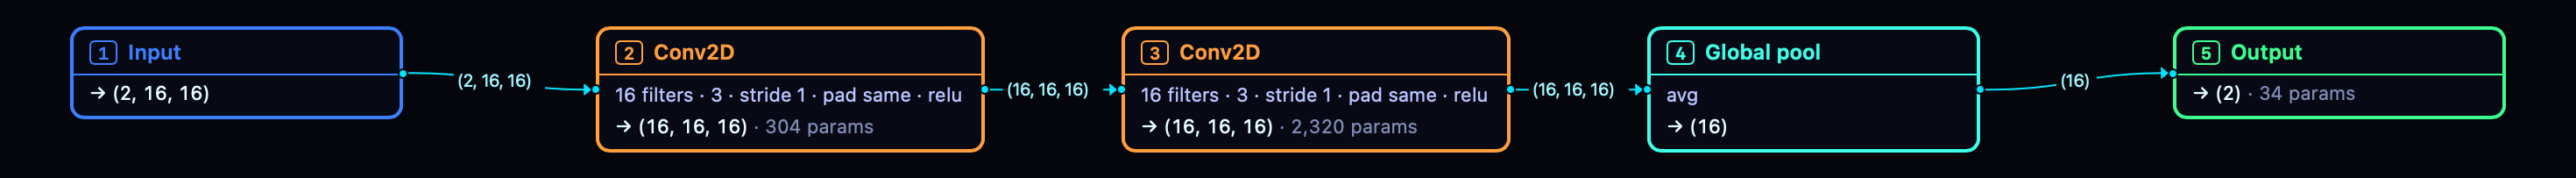
\includegraphics[width=\linewidth,height=0.55\textheight,keepaspectratio]{figures/tests/test10_arch.png}\caption{TEST 10 as a picture: \ui{Save as PNG} on the Design screen (or \ui{File} $\rightarrow$ \ui{Export Design as PNG}) draws the whole design at full size; long designs are split into rows here to fit the page.}\label{fig:test10arch}\end{figure}

The network is plain (304 + 2\,320 + 34 = 2\,658 parameters); the test is in the Train tab: \emph{inverse} class weights (0.55 for the common class, 5.5 for the rare one, so each class counts as much in total) and focal loss. Read folder in the Dataset tab showed the 10:1 imbalance and suggested the weights.

{\small
\begin{longtable}{@{}lp{3.2cm}p{5.4cm}lr@{}}
\toprule
\textbf{Id} & \textbf{Block} & \textbf{Settings} & \textbf{Output} & \textbf{Parameters}\\
\midrule\endhead
t1 & Input & all bands & $2\times16\times16$ & 0\\
t2 & Conv2D & 16 filters, $3\times3$, same, relu & $16\times16\times16$ & 304\\
t3 & Conv2D & 16 filters, $3\times3$, same, relu & $16\times16\times16$ & 2\,320\\
t4 & Global pool & avg & $16$ & 0\\
t5 & Output & main output & $2$ & 34\\
\midrule
 & \textbf{Total} & & & \textbf{2\,658}\\
\bottomrule
\end{longtable}}

\subsection{TEST 11: ViT-B/16 fine-tuned with LoRA}
\label{sec:test11}

TEST 11 and TEST 12 start from the same ViT-B/16 with ImageNet weights and fine-tune it on EuroSAT RGB (1 epoch, 4\,000 images); TEST 11 adapts it with LoRA, TEST 12 trains everything.

\screenshot{figures/tests/test11.jpg}{TEST 11 on the Design screen: the ViT-B/16 demo with its 12 encoder blocks collapsed (\ui{Collapse repeated blocks}).}{fig:test11}

\begin{figure}[htbp]\centering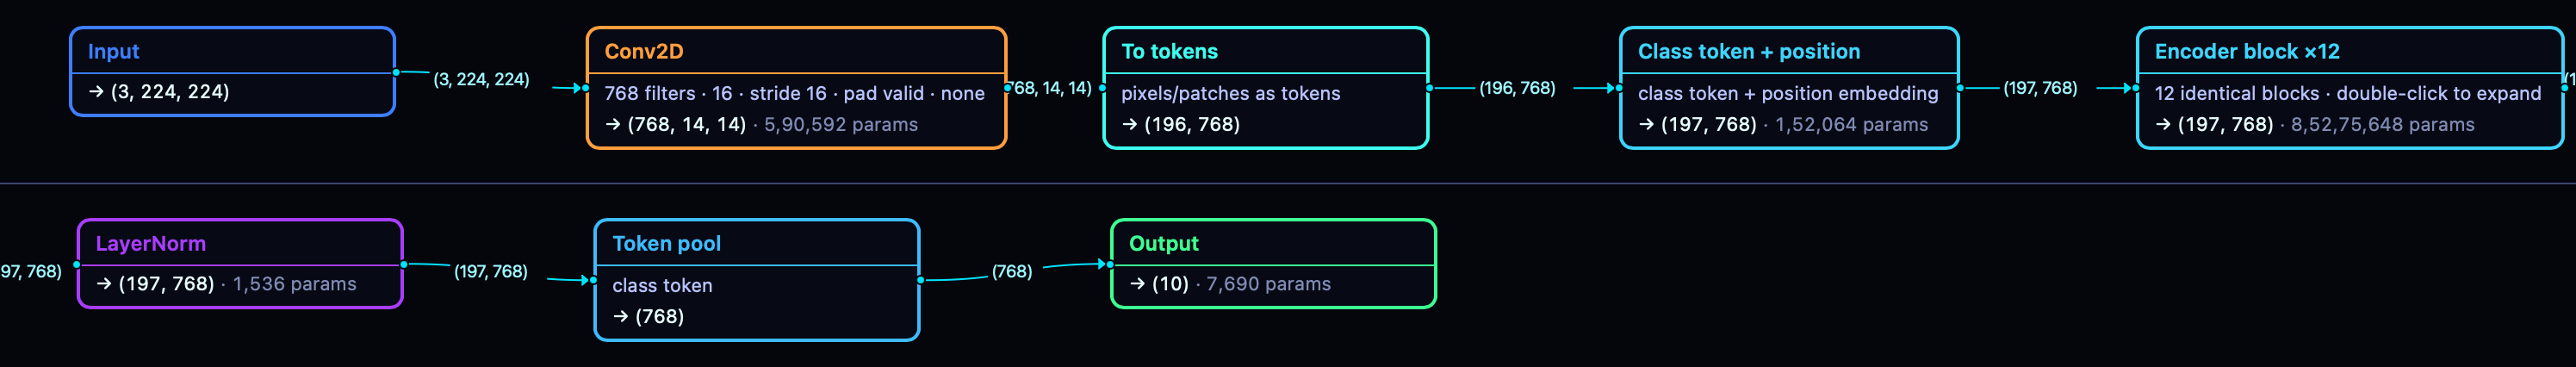
\includegraphics[width=\linewidth,height=0.55\textheight,keepaspectratio]{figures/tests/test11_arch.png}\caption{TEST 11 as a picture: \ui{Save as PNG} on the Design screen (or \ui{File} $\rightarrow$ \ui{Export Design as PNG}) draws the whole design at full size, with the repeated encoder blocks collapsed; long designs are split into rows here to fit the page.}\label{fig:test11arch}\end{figure}

ViT-B/16 cuts the 224$\times$224 image into 196 patches with a 16$\times$16 convolution ($16\cdot16\cdot3\cdot768+768=590\,592$), adds a class token and 197 learned positions ($768+197\cdot768=152\,064$) and runs 12 encoder blocks. Each block has two LayerNorms, a self-attention ($4\cdot768^2+4\cdot768=2\,362\,368$) and a two-layer MLP ($768\cdot3072+3072+3072\cdot768+768=4\,722\,432$). Here every attention has LoRA rank 4 on q, k and v: $3\cdot4\cdot(768+768)=18\,432$ new weights per block, 221\,184 in all, while the 28\,348\,416 attention weights are frozen. With \ui{Train: backbone} the run also keeps every other ImageNet weight fixed, so only the adapters and the new 10-class Output ($768\cdot10+10=7\,690$) learn: 228\,874 weights, 0.27\,\% of the network, for 93.6\,\% after one epoch.

{\small
\begin{longtable}{@{}lrrr@{}}
\toprule
\textbf{Block kind} & \textbf{Blocks} & \textbf{Parameters} & \textbf{of them frozen}\\
\midrule\endhead
Input & 1 & 0 & --\\
Conv2D & 1 & 590\,592 & --\\
To tokens & 1 & 0 & --\\
Class token + positions & 1 & 152\,064 & --\\
LayerNorm & 25 & 38\,400 & --\\
Self-attention & 12 & 28\,569\,600 & 28\,348\,416\\
Add & 24 & 0 & --\\
Dense & 24 & 56\,669\,184 & --\\
Token pool & 1 & 0 & --\\
Output & 1 & 7\,690 & --\\
\midrule
\textbf{Total} & 91 & \textbf{86\,027\,530} & 28\,348\,416\\
\bottomrule
\end{longtable}}

\subsection{TEST 12: ViT-B/16, full fine-tuning}
\label{sec:test12}

TEST 12 is TEST 11 without LoRA: all 85\,806\,346 weights are trained.

\screenshot{figures/tests/test12.jpg}{TEST 12 on the Design screen: the same ViT-B/16, collapsed.}{fig:test12}

\begin{figure}[htbp]\centering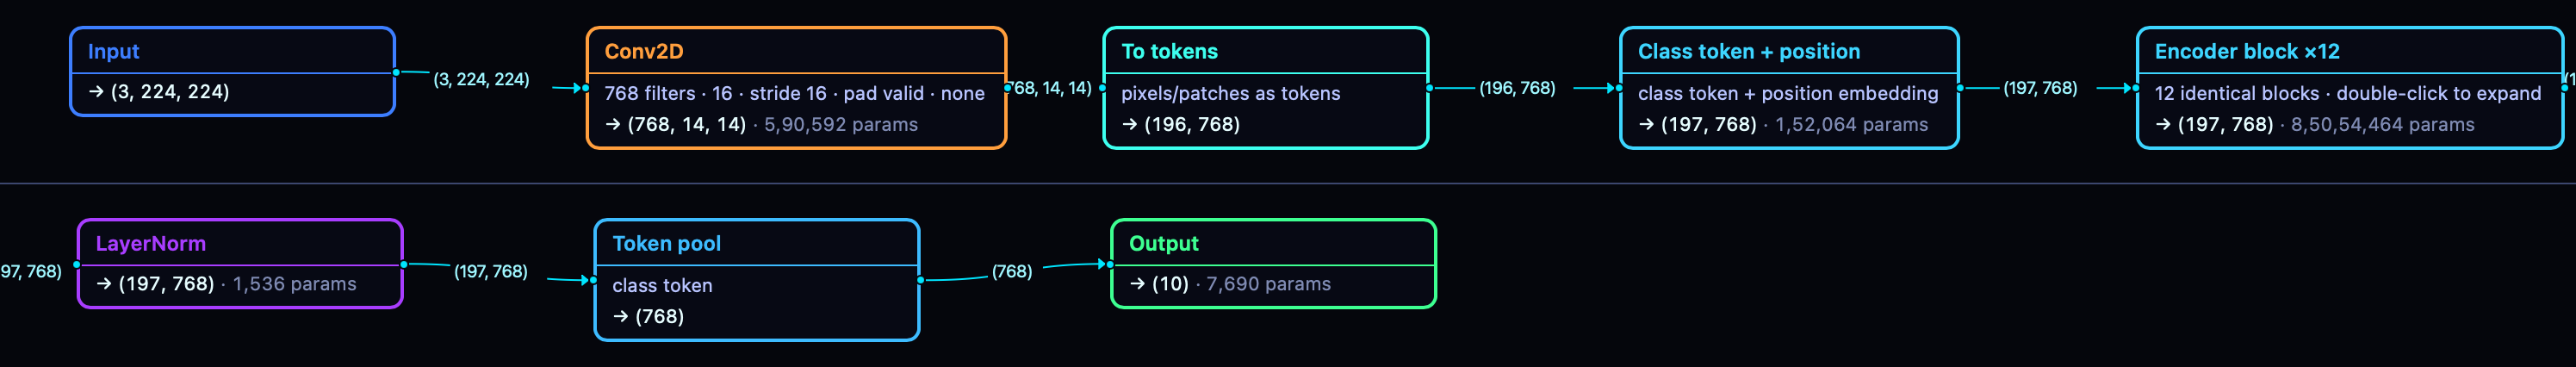
\includegraphics[width=\linewidth,height=0.55\textheight,keepaspectratio]{figures/tests/test12_arch.png}\caption{TEST 12 as a picture: \ui{Save as PNG} on the Design screen (or \ui{File} $\rightarrow$ \ui{Export Design as PNG}) draws the whole design at full size, with the repeated encoder blocks collapsed; long designs are split into rows here to fit the page.}\label{fig:test12arch}\end{figure}

The difference to TEST 11 is exactly the LoRA adapters ($86\,027\,530 - 85\,806\,346 = 221\,184$). Full fine-tuning reached 96.8\,\% against LoRA's 93.6\,\% in the same single epoch and about the same time (100\,s per epoch on a T4); LoRA trains 375 times fewer weights and its checkpoints are correspondingly small. The MLPs (56.7 M) hold two thirds of the parameters, the attention layers one third.

{\small
\begin{longtable}{@{}lrrr@{}}
\toprule
\textbf{Block kind} & \textbf{Blocks} & \textbf{Parameters} & \textbf{of them frozen}\\
\midrule\endhead
Input & 1 & 0 & --\\
Conv2D & 1 & 590\,592 & --\\
To tokens & 1 & 0 & --\\
Class token + positions & 1 & 152\,064 & --\\
LayerNorm & 25 & 38\,400 & --\\
Self-attention & 12 & 28\,348\,416 & --\\
Add & 24 & 0 & --\\
Dense & 24 & 56\,669\,184 & --\\
Token pool & 1 & 0 & --\\
Output & 1 & 7\,690 & --\\
\midrule
\textbf{Total} & 91 & \textbf{85\,806\,346} & --\\
\bottomrule
\end{longtable}}

\subsection{TEST 13: every block of the language}
\label{sec:test13}

TEST 13 trains \file{doc/examples/everything.nnb}, the design text that uses every block kind and language feature, on CIFAR-10 with the recommended recipe, three seeds, \ui{save memory} and the TorchScript / ONNX export.

\screenshot{figures/tests/test13.jpg}{TEST 13 on the Design screen: the 97 blocks of \file{everything.nnb} (the canvas shows it from far; the layer table groups it).}{fig:test13}

\begin{figure}[htbp]\centering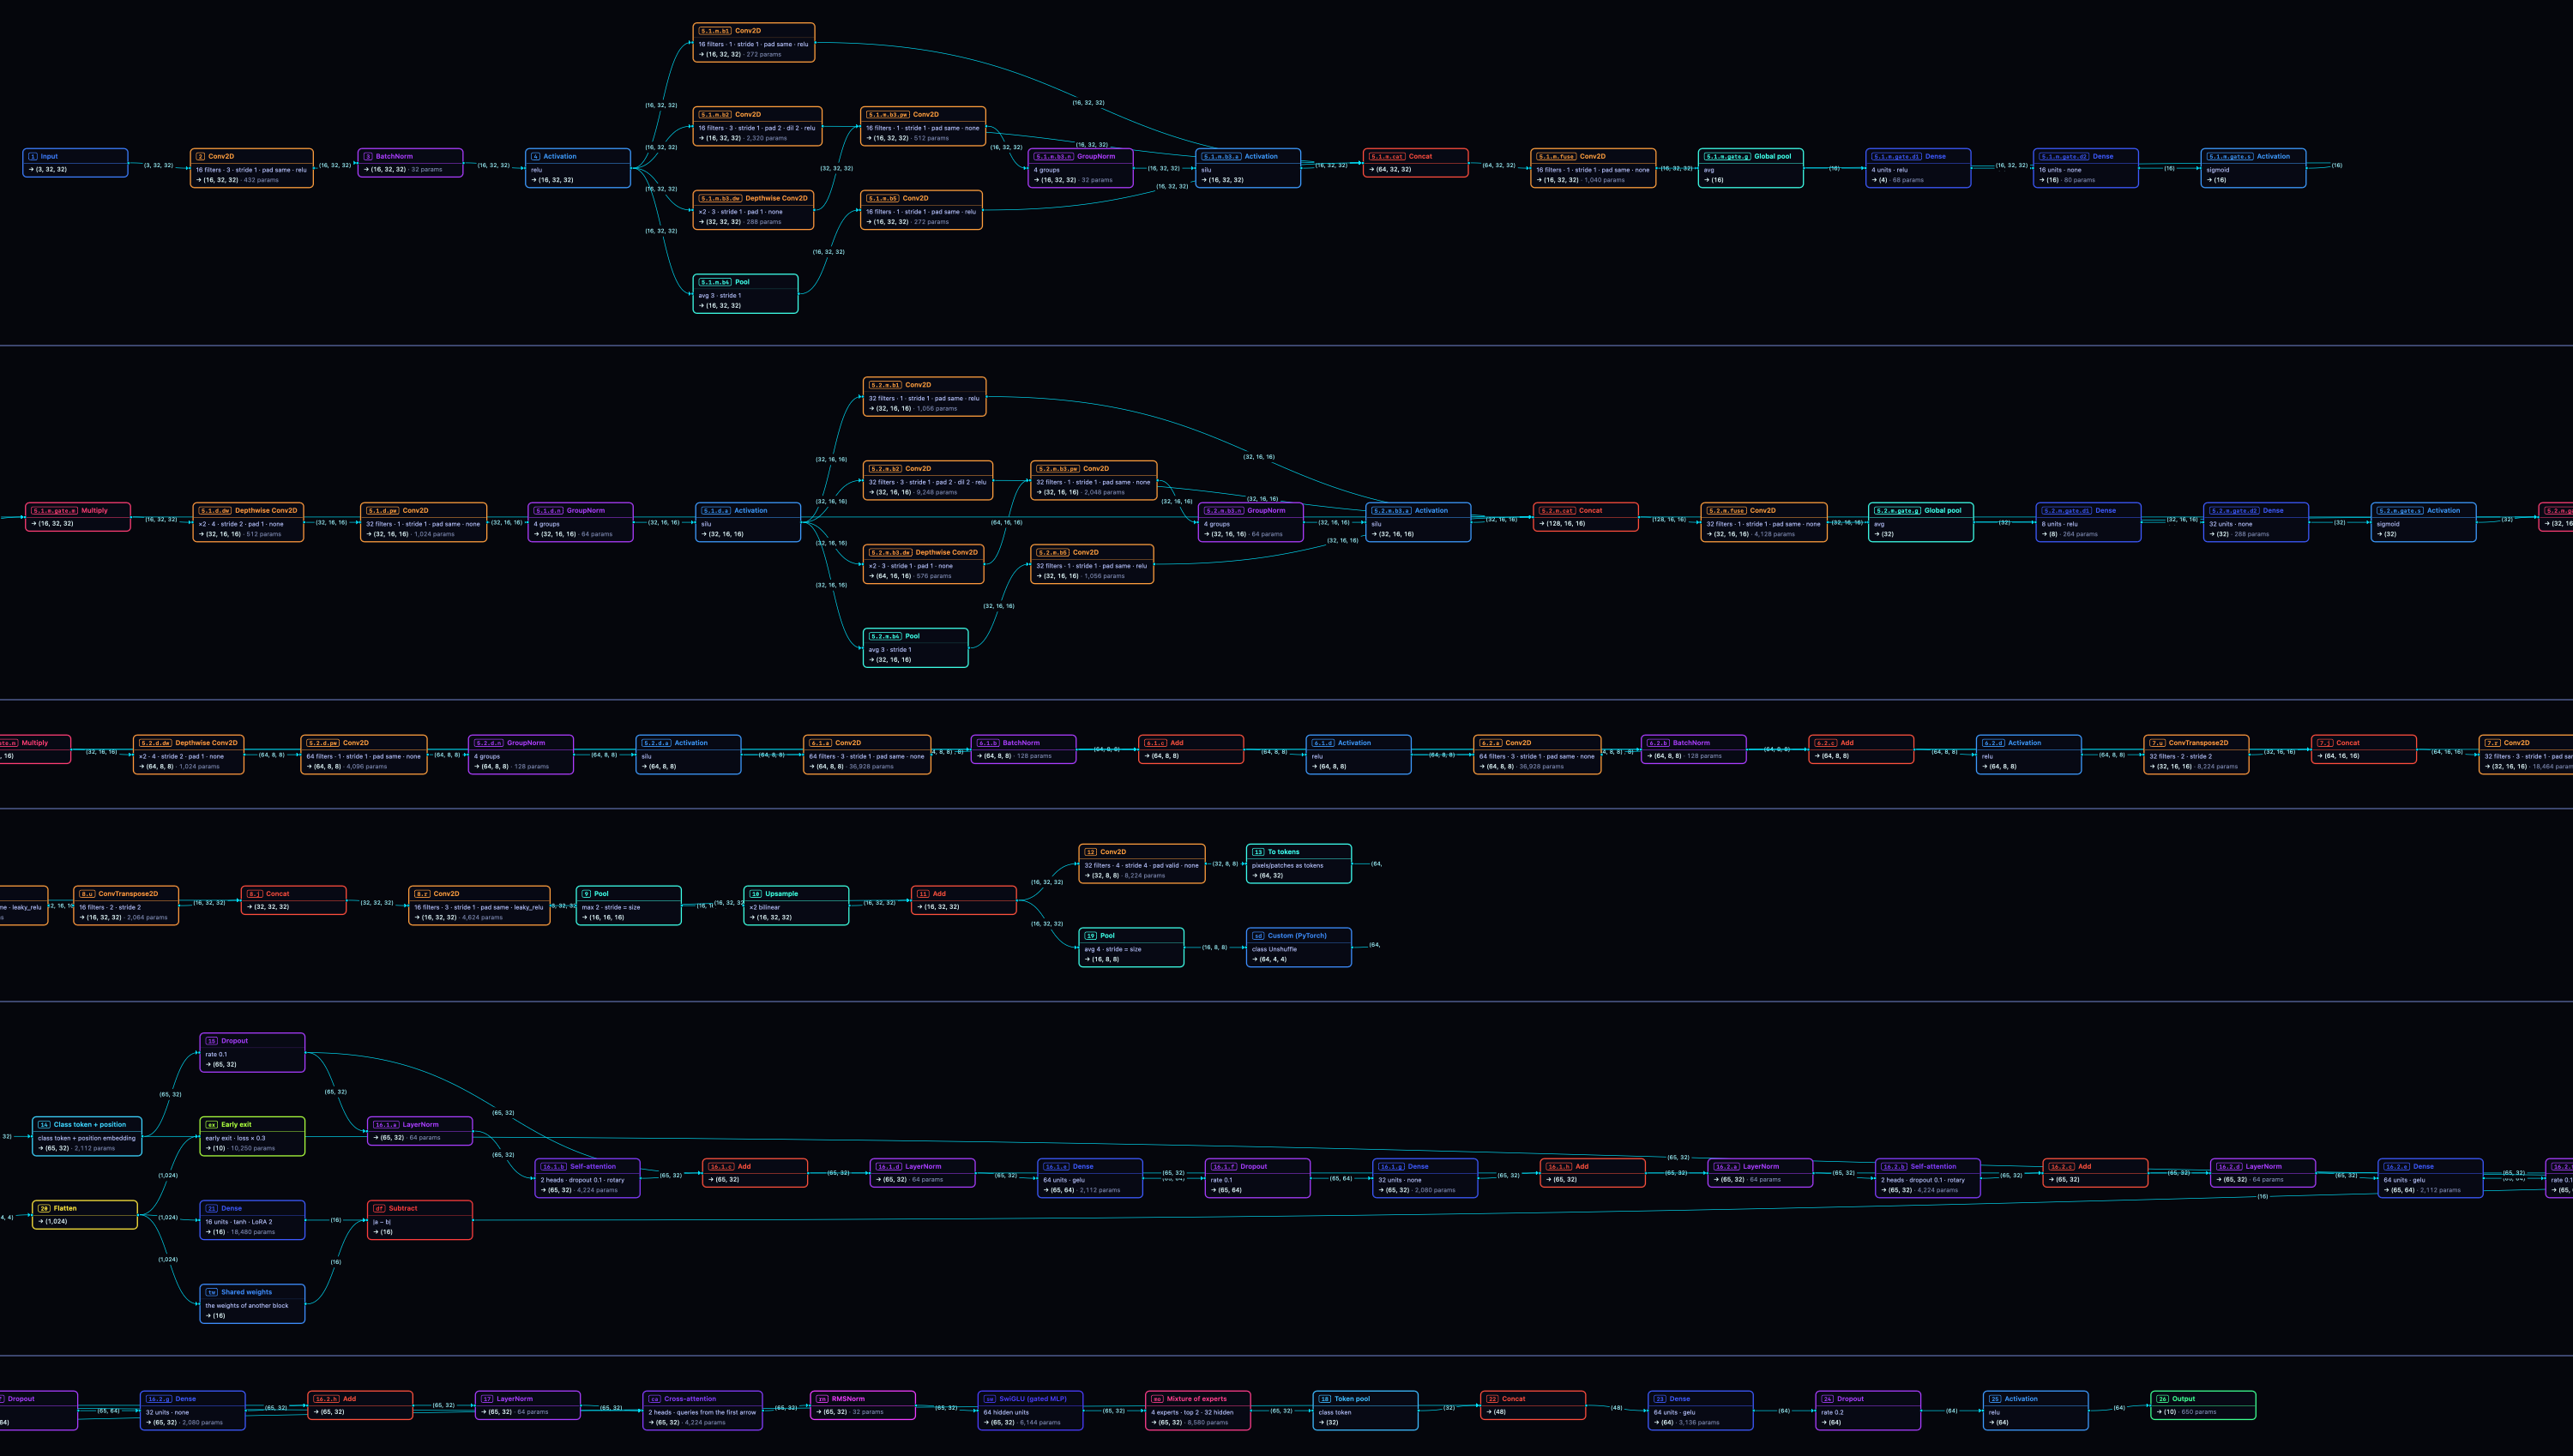
\includegraphics[width=\linewidth,height=0.55\textheight,keepaspectratio]{figures/tests/test13_arch.png}\caption{TEST 13 as a picture: \ui{Save as PNG} on the Design screen (or \ui{File} $\rightarrow$ \ui{Export Design as PNG}) draws the whole design at full size; long designs are split into rows here to fit the page.}\label{fig:test13arch}\end{figure}

It is a test of breadth, not a good classifier: Inception-like branches, depthwise convolutions, GroupNorm, a squeeze-and-excitation gate (Multiply), a U-Net style up-sampling path, a Custom block, a frozen convolution, shared weights with Subtract, attention with cross-attention, RMSNorm, SwiGLU, a mixture of experts, a LoRA Dense and an early exit. The table groups its 97 blocks by kind. 16\,832 parameters are frozen (a frozen 3$\times$3 convolution, 432, and the base of the LoRA Dense, 16\,400). Three seeds of two epochs each gave 49.30, 52.53 and 51.01\,\%: mean 50.95\,\%, sample standard deviation 1.62 points, which the Compare panel and the exported LaTeX table report.

{\small
\begin{longtable}{@{}lrrr@{}}
\toprule
\textbf{Block kind} & \textbf{Blocks} & \textbf{Parameters} & \textbf{of them frozen}\\
\midrule\endhead
Input & 1 & 0 & --\\
Conv2D & 18 & 132\,672 & 432\\
BatchNorm & 3 & 288 & --\\
Activation & 10 & 0 & --\\
Depthwise Conv2D & 4 & 2\,400 & --\\
Pool & 4 & 0 & --\\
groupnorm & 4 & 288 & --\\
Concat & 5 & 0 & --\\
Global pool & 2 & 0 & --\\
Dense & 10 & 30\,700 & 16\,400\\
multiply & 2 & 0 & --\\
Add & 7 & 0 & --\\
convtranspose2d & 2 & 10\,288 & --\\
upsample & 1 & 0 & --\\
To tokens & 1 & 0 & --\\
Custom (PyTorch) & 1 & 0 & --\\
Class token + positions & 1 & 2\,112 & --\\
Flatten & 1 & 0 & --\\
Dropout & 4 & 0 & --\\
Early exit & 1 & 10\,250 & --\\
LayerNorm & 5 & 320 & --\\
Shared weights & 1 & 0 & --\\
Self-attention & 2 & 8\,448 & --\\
Subtract & 1 & 0 & --\\
cross\_attention & 1 & 4\,224 & --\\
RMSNorm & 1 & 32 & --\\
SwiGLU & 1 & 6\,144 & --\\
Mixture of experts & 1 & 8\,580 & --\\
Token pool & 1 & 0 & --\\
Output & 1 & 650 & --\\
\midrule
\textbf{Total} & 97 & \textbf{217\,396} & 16\,832\\
\bottomrule
\end{longtable}}

\subsection{TEST 14: a time series written as text}
\label{sec:test14}

TEST 14 is \file{doc/examples/timeseries.nnb} pasted into the Text tab, with one setting changed on the canvas (the LSTM from 16 to 24 units) to check that only that line of the text changes.

\screenshot{figures/tests/test14.jpg}{TEST 14 on the Design screen: two paths from the same input: Conv3D + temporal attention (image path) and a sequence path with Conv1D, LSTM, GRU and attention.}{fig:test14}

\begin{figure}[htbp]\centering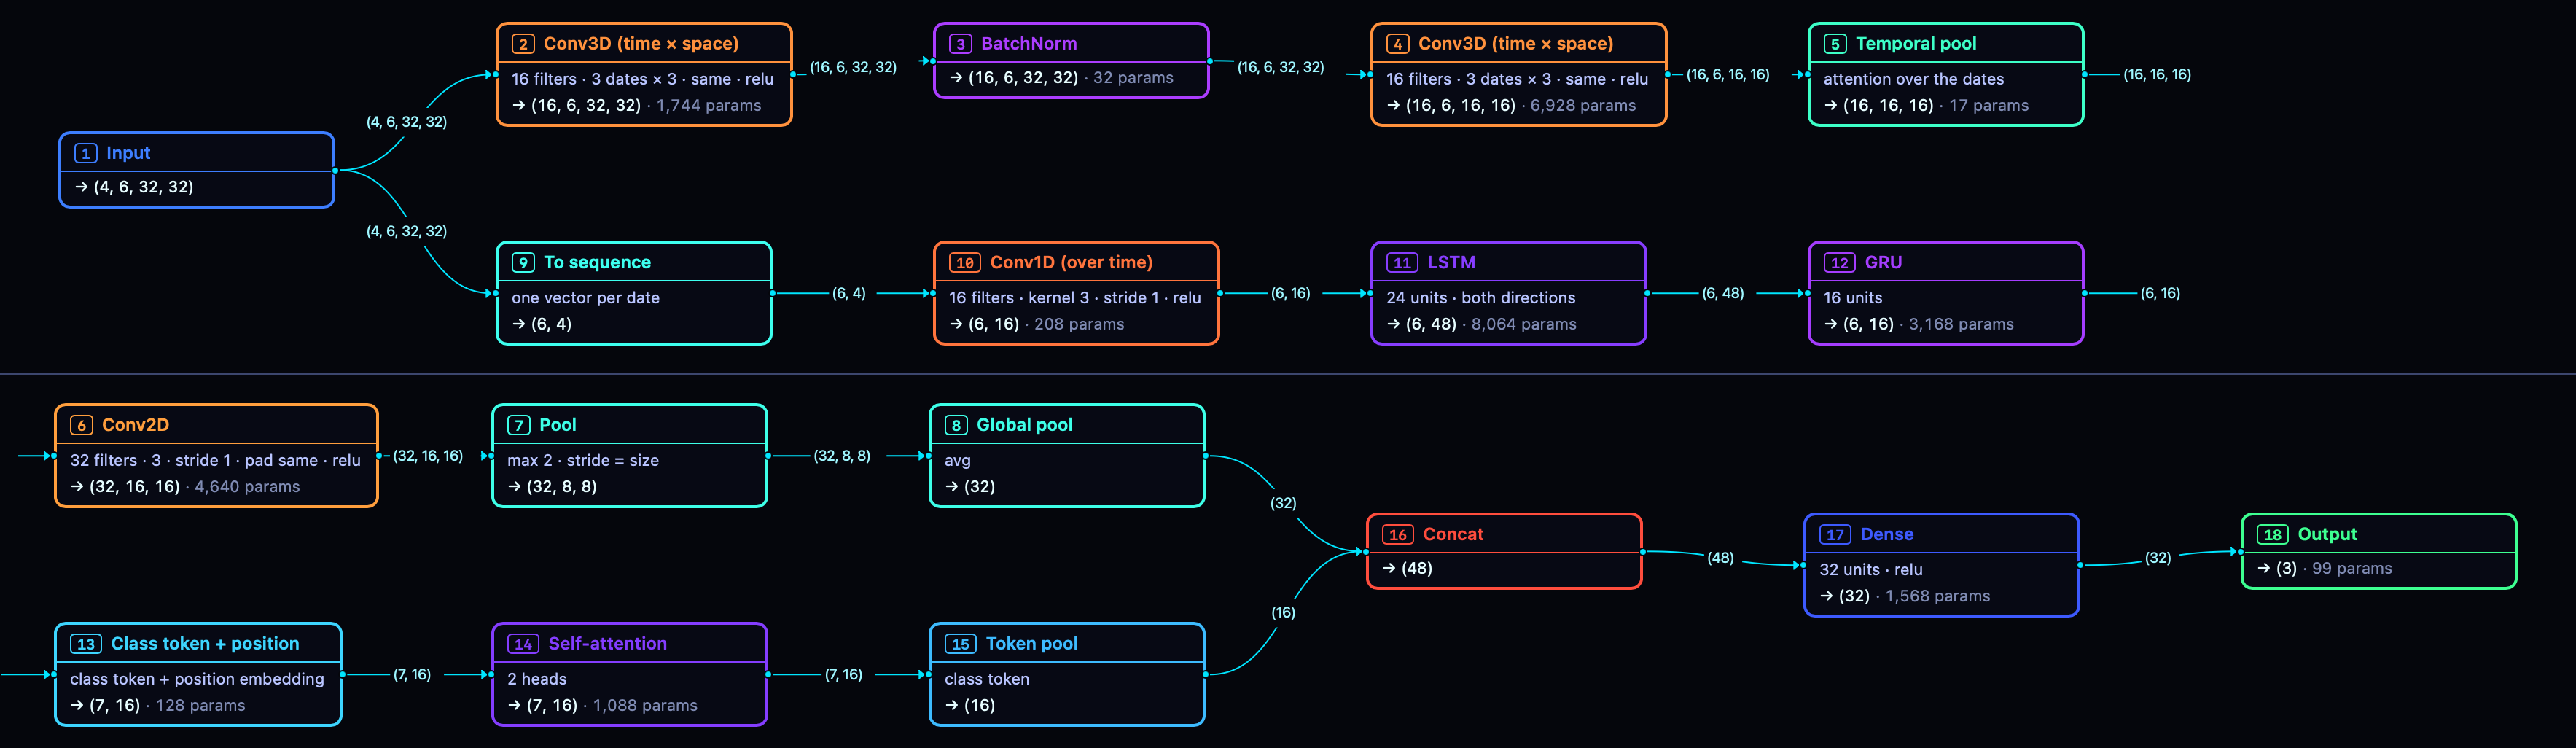
\includegraphics[width=\linewidth,height=0.55\textheight,keepaspectratio]{figures/tests/test14_arch.png}\caption{TEST 14 as a picture: \ui{Save as PNG} on the Design screen (or \ui{File} $\rightarrow$ \ui{Export Design as PNG}) draws the whole design at full size; long designs are split into rows here to fit the page.}\label{fig:test14arch}\end{figure}

The input is 4 bands $\times$ 6 dates $\times$ 32$\times$32 pixels. The \emph{image path} (U-TAE style) runs two Conv3D layers (1\,744 and 6\,928), weighs the dates per pixel with temporal attention, and ends in a 2-D convolution (4\,640) and a global pool. The \emph{sequence path} (TSViT style) averages each date into a 4-number vector, then Conv1D ($3\cdot4\cdot16+16=208$), a bidirectional LSTM of 24 units ($2\cdot4\cdot(16\cdot24+24^2+2\cdot24)=8\,064$, the largest block after the edit), a GRU ($3\cdot(48\cdot16+16^2+2\cdot16)=3\,168$) and a small transformer step (class token and 7 learned positions, 128; attention, 1\,088). Concat joins the 32 + 16 numbers for the Dense and the Output.

{\small
\begin{longtable}{@{}lp{3.2cm}p{5.4cm}lr@{}}
\toprule
\textbf{Id} & \textbf{Block} & \textbf{Settings} & \textbf{Output} & \textbf{Parameters}\\
\midrule\endhead
t1 & Input & all bands & $4\times6\times32\times32$ & 0\\
t2\_2 & Conv3D & 16 filters, $3\times3$ over 3 dates, relu & $16\times6\times32\times32$ & 1\,744\\
t9 & To sequence &  & $6\times4$ & 0\\
t3\_2 & BatchNorm &  & $16\times6\times32\times32$ & 32\\
t10 & Conv1D & 16 filters, kernel 3, relu & $6\times16$ & 208\\
t4\_2 & Conv3D & 16 filters, $3\times3$ over 3 dates, stride 2, relu & $16\times6\times16\times16$ & 6\,928\\
t11 & LSTM & 24 units, both directions & $6\times48$ & 8\,064\\
t5 & Temporal pool & attention & $16\times16\times16$ & 17\\
t12 & GRU & 16 units & $6\times16$ & 3\,168\\
t6 & Conv2D & 32 filters, $3\times3$, same, relu & $32\times16\times16$ & 4\,640\\
t13 & Class token + positions & positions learned & $7\times16$ & 128\\
t7 & Pool & max 2$\times$2 & $32\times8\times8$ & 0\\
t14 & Self-attention & 2 heads & $7\times16$ & 1\,088\\
t8 & Global pool & avg & $32$ & 0\\
t15 & Token pool & cls & $16$ & 0\\
t16 & Concat &  & $48$ & 0\\
t17 & Dense & 32 units, relu & $32$ & 1\,568\\
t18 & Output & main output & $3$ & 99\\
\midrule
 & \textbf{Total} & & & \textbf{27\,684}\\
\bottomrule
\end{longtable}}

\subsection{TEST 15: segmentation of a large scene}
\label{sec:test15}

TEST 15 trains on one large generated scene with a label image on the same grid, cut into 16$\times$16 tiles; the test tiles are the eastern strip, with a column of tiles left out in between so that training and test pixels never touch.

\screenshot{figures/tests/test15.jpg}{TEST 15 on the Design screen: two convolutions and the Segmentation output.}{fig:test15}

\begin{figure}[htbp]\centering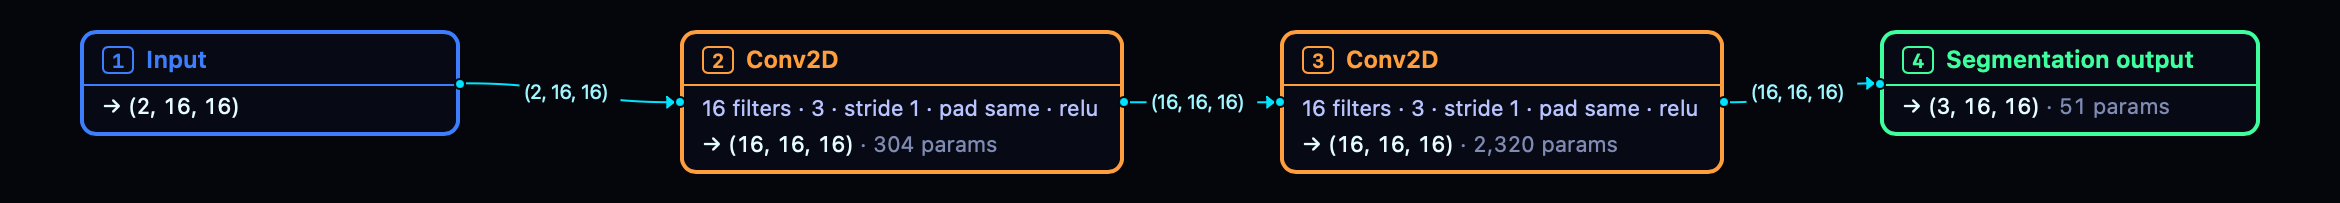
\includegraphics[width=\linewidth,height=0.55\textheight,keepaspectratio]{figures/tests/test15_arch.png}\caption{TEST 15 as a picture: \ui{Save as PNG} on the Design screen (or \ui{File} $\rightarrow$ \ui{Export Design as PNG}) draws the whole design at full size; long designs are split into rows here to fit the page.}\label{fig:test15arch}\end{figure}

A minimal fully convolutional network: two 3$\times$3 convolutions (304 and 2\,320) keep the full resolution, and the Segmentation output (1$\times$1, $16\cdot3+3=51$) gives three class scores per pixel. Being fully convolutional, the same 2\,675 weights work on any tile size.

{\small
\begin{longtable}{@{}lp{3.2cm}p{5.4cm}lr@{}}
\toprule
\textbf{Id} & \textbf{Block} & \textbf{Settings} & \textbf{Output} & \textbf{Parameters}\\
\midrule\endhead
t1 & Input & all bands & $2\times16\times16$ & 0\\
t2 & Conv2D & 16 filters, $3\times3$, same, relu & $16\times16\times16$ & 304\\
t3 & Conv2D & 16 filters, $3\times3$, same, relu & $16\times16\times16$ & 2\,320\\
t4 & Segmentation output &  & $3\times16\times16$ & 51\\
\midrule
 & \textbf{Total} & & & \textbf{2\,675}\\
\bottomrule
\end{longtable}}

\subsection{TEST 16: the Small CNN on AWS}
\label{sec:test16}

TEST 16 is the Small CNN demo, used to test training on Amazon EC2: start and stop of the instance, Prepare, fetching results from a stopped instance, the app closed during a run, and Stop.

\screenshot{figures/tests/test16.jpg}{TEST 16 on the Design screen: the Small CNN (CIFAR-10) demo: three VGG-style stages and a Dense classifier.}{fig:test16}

\begin{figure}[htbp]\centering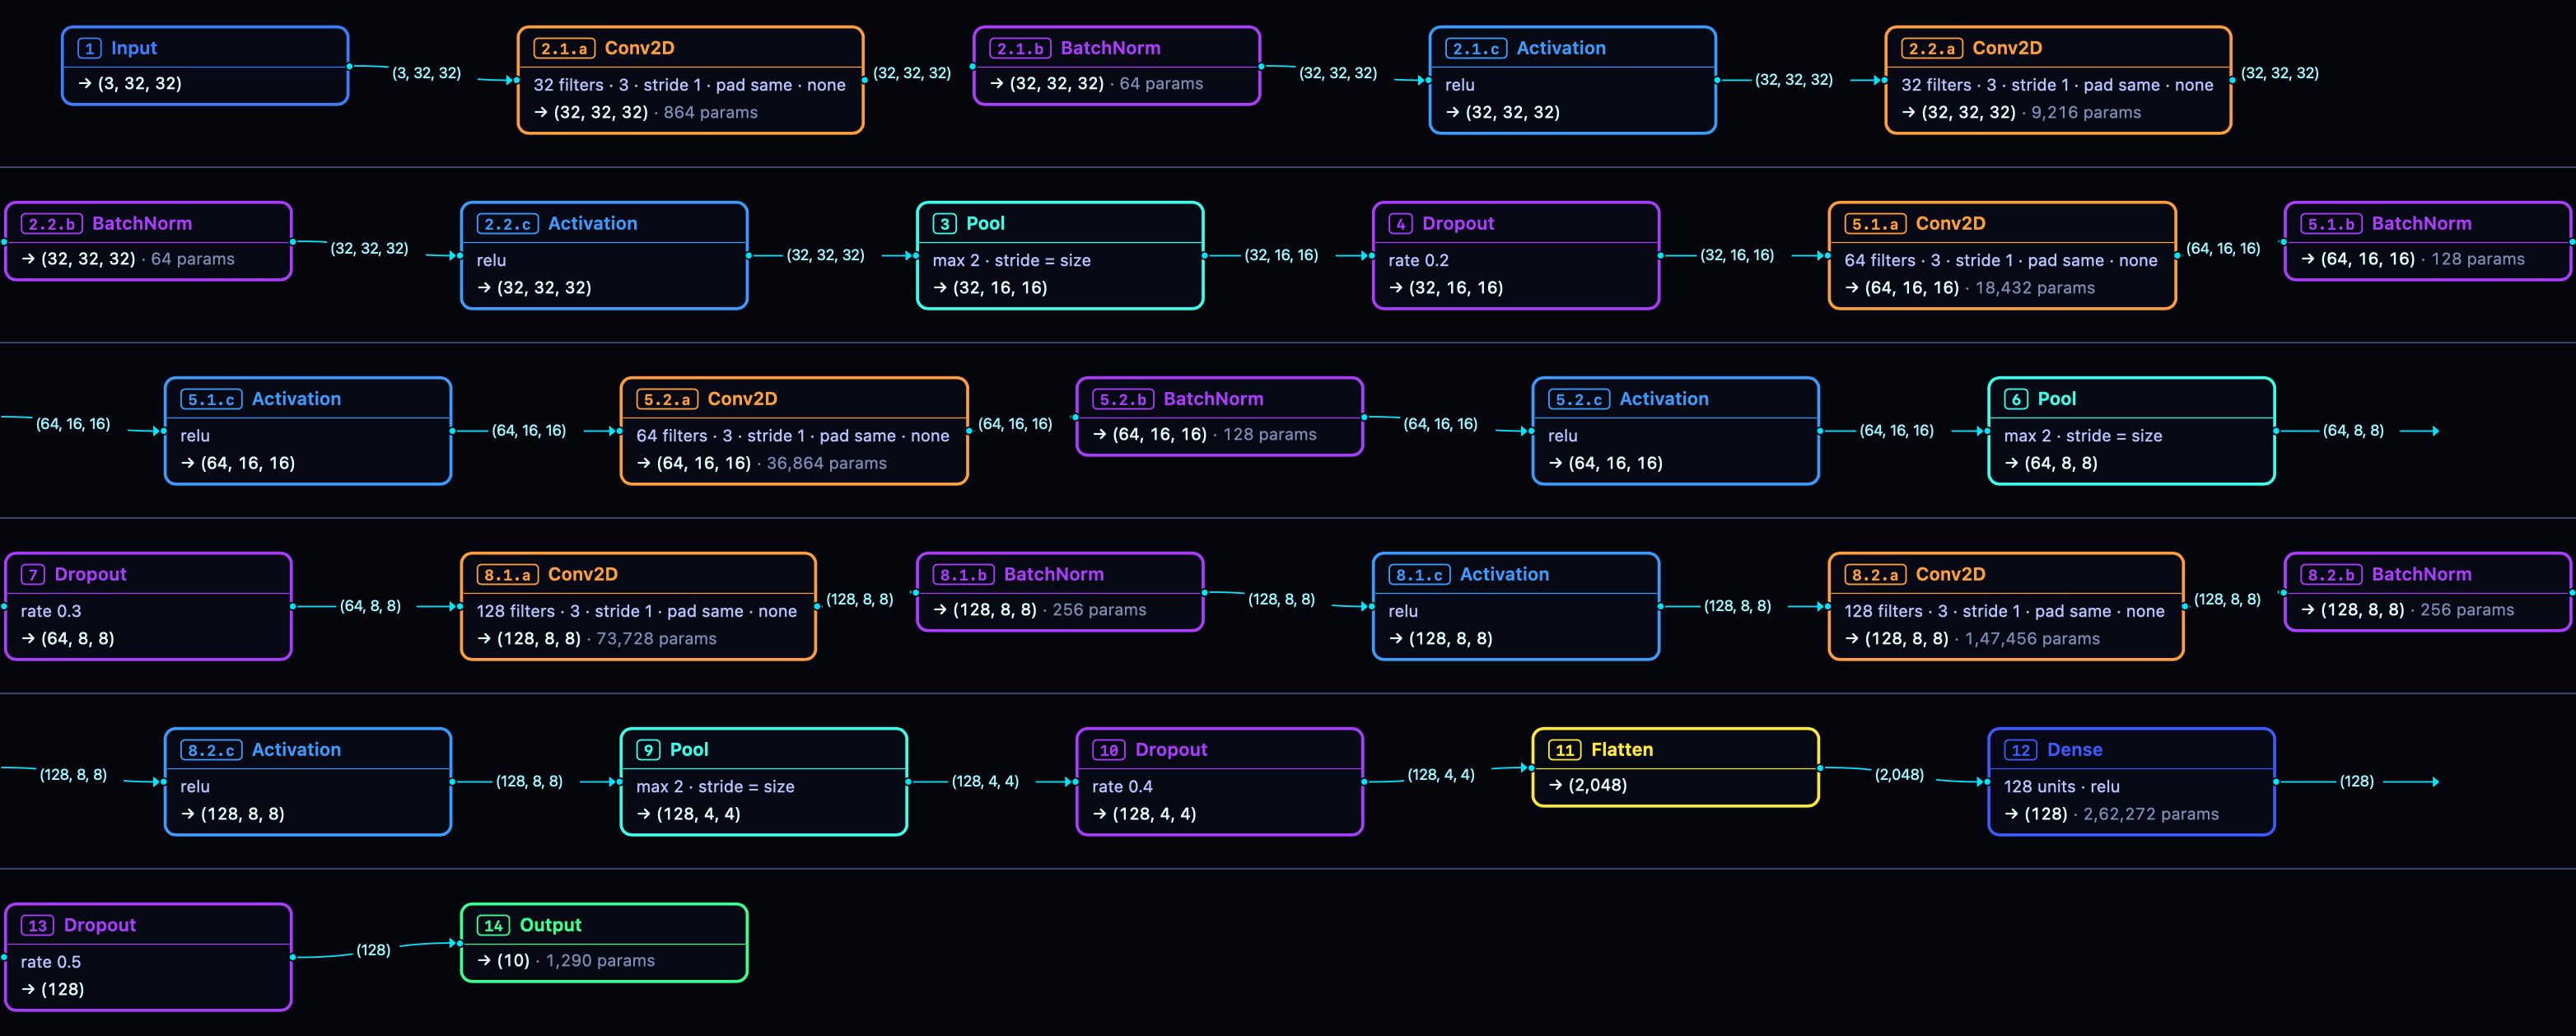
\includegraphics[width=\linewidth,height=0.55\textheight,keepaspectratio]{figures/tests/test16_arch.png}\caption{TEST 16 as a picture: \ui{Save as PNG} on the Design screen (or \ui{File} $\rightarrow$ \ui{Export Design as PNG}) draws the whole design at full size; long designs are split into rows here to fit the page.}\label{fig:test16arch}\end{figure}

Three stages of two 3$\times$3 convolutions (without biases, as BatchNorm follows) at 32, 64 and 128 channels; each stage ends in max pooling and dropout. The convolutions grow from 864 to 147\,456 weights, but the largest block is the Dense layer after Flatten: $2\,048\cdot128+128=262\,272$, almost half of the 551\,018. That is typical of CNNs that flatten instead of pooling globally.

{\small
\begin{longtable}{@{}lp{3.2cm}p{5.4cm}lr@{}}
\toprule
\textbf{Id} & \textbf{Block} & \textbf{Settings} & \textbf{Output} & \textbf{Parameters}\\
\midrule\endhead
n1 & Input & all bands & $3\times32\times32$ & 0\\
n2 & Conv2D & 32 filters, $3\times3$, same & $32\times32\times32$ & 864\\
n3 & BatchNorm &  & $32\times32\times32$ & 64\\
n4 & Activation & relu & $32\times32\times32$ & 0\\
n5 & Conv2D & 32 filters, $3\times3$, same & $32\times32\times32$ & 9\,216\\
n6 & BatchNorm &  & $32\times32\times32$ & 64\\
n7 & Activation & relu & $32\times32\times32$ & 0\\
n8 & Pool & max 2$\times$2 & $32\times16\times16$ & 0\\
n9 & Dropout & rate 0.2 & $32\times16\times16$ & 0\\
n10 & Conv2D & 64 filters, $3\times3$, same & $64\times16\times16$ & 18\,432\\
n11 & BatchNorm &  & $64\times16\times16$ & 128\\
n12 & Activation & relu & $64\times16\times16$ & 0\\
n13 & Conv2D & 64 filters, $3\times3$, same & $64\times16\times16$ & 36\,864\\
n14 & BatchNorm &  & $64\times16\times16$ & 128\\
n15 & Activation & relu & $64\times16\times16$ & 0\\
n16 & Pool & max 2$\times$2 & $64\times8\times8$ & 0\\
n17 & Dropout & rate 0.3 & $64\times8\times8$ & 0\\
n18 & Conv2D & 128 filters, $3\times3$, same & $128\times8\times8$ & 73\,728\\
n19 & BatchNorm &  & $128\times8\times8$ & 256\\
n20 & Activation & relu & $128\times8\times8$ & 0\\
n21 & Conv2D & 128 filters, $3\times3$, same & $128\times8\times8$ & 147\,456\\
n22 & BatchNorm &  & $128\times8\times8$ & 256\\
n23 & Activation & relu & $128\times8\times8$ & 0\\
n24 & Pool & max 2$\times$2 & $128\times4\times4$ & 0\\
n25 & Dropout & rate 0.4 & $128\times4\times4$ & 0\\
n26 & Flatten &  & $2048$ & 0\\
n27 & Dense & 128 units, relu & $128$ & 262\,272\\
n28 & Dropout & rate 0.5 & $128$ & 0\\
n29 & Output & main output & $10$ & 1\,290\\
\midrule
 & \textbf{Total} & & & \textbf{551\,018}\\
\bottomrule
\end{longtable}}

\subsection{TEST 17: real Earth Engine exports, S2 + S1}
\label{sec:test17}

TEST 17 reads 40 real Sentinel-1 / Sentinel-2 image pairs exported from Google Earth Engine (S2 Level-1C, 13 bands; S1 VV and VH in dB; LZW-compressed GeoTIFFs) and checks them on Kaggle.

\screenshot{figures/tests/test17.jpg}{TEST 17 on the Design screen: an early-fusion CNN on 15 channels.}{fig:test17}

\begin{figure}[htbp]\centering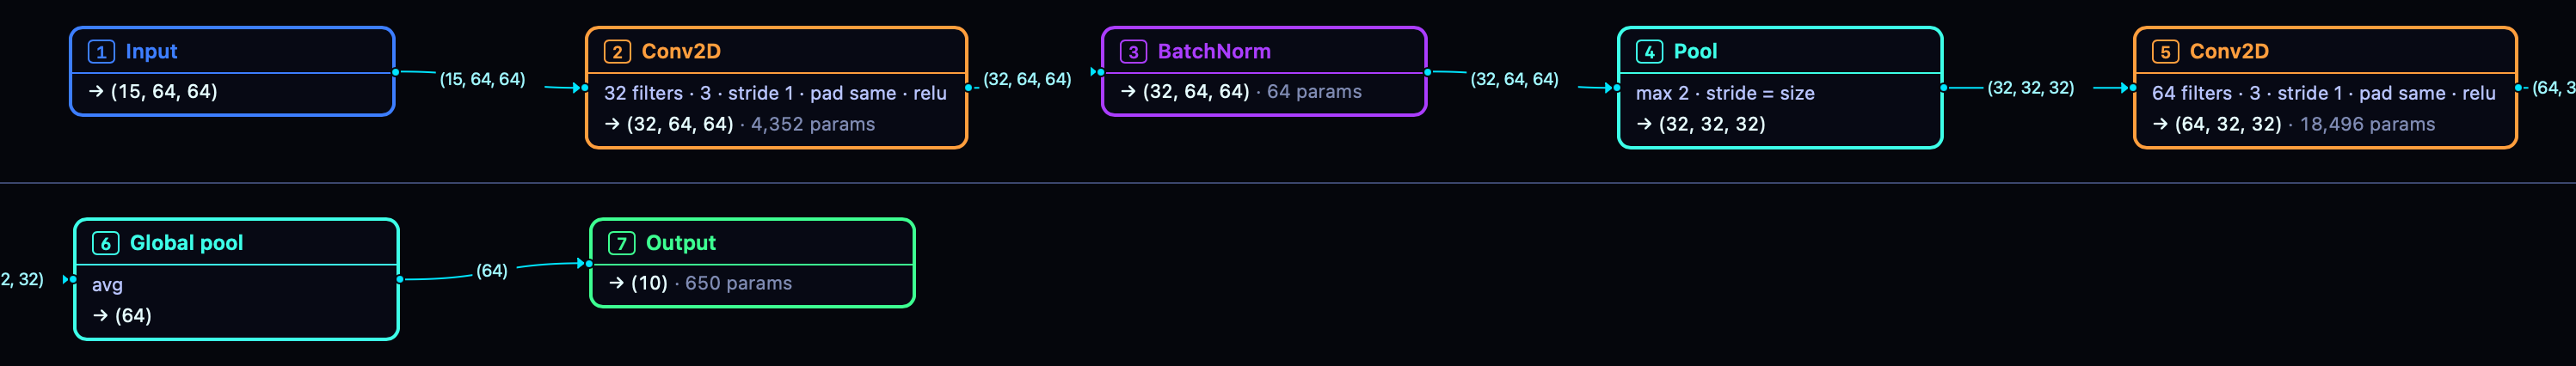
\includegraphics[width=\linewidth,height=0.55\textheight,keepaspectratio]{figures/tests/test17_arch.png}\caption{TEST 17 as a picture: \ui{Save as PNG} on the Design screen (or \ui{File} $\rightarrow$ \ui{Export Design as PNG}) draws the whole design at full size; long designs are split into rows here to fit the page.}\label{fig:test17arch}\end{figure}

The two groups are stacked into 15 channels (13 + 2), so the first convolution has $3\cdot3\cdot15\cdot32+32=4\,352$ weights. The data check read every pair, confirmed the radar was already in decibels (VV mean $-13.3$\,dB, VH $-21.6$\,dB) and passed one batch of 2$\times$15$\times$64$\times$64 through the network. Testing it found four bugs (LZW files on Kaggle, the band names of the second group, a 13-band header and a full path as the second group's folder), all fixed.

{\small
\begin{longtable}{@{}lp{3.2cm}p{5.4cm}lr@{}}
\toprule
\textbf{Id} & \textbf{Block} & \textbf{Settings} & \textbf{Output} & \textbf{Parameters}\\
\midrule\endhead
t1 & Input & all bands & $15\times64\times64$ & 0\\
t2 & Conv2D & 32 filters, $3\times3$, same, relu & $32\times64\times64$ & 4\,352\\
t3 & BatchNorm &  & $32\times64\times64$ & 64\\
t4 & Pool & max 2$\times$2 & $32\times32\times32$ & 0\\
t5 & Conv2D & 64 filters, $3\times3$, same, relu & $64\times32\times32$ & 18\,496\\
t6 & Global pool & avg & $64$ & 0\\
t7 & Output & main output & $10$ & 650\\
\midrule
 & \textbf{Total} & & & \textbf{23\,562}\\
\bottomrule
\end{longtable}}

\subsection{TEST 19: the app's Earth Engine export}
\label{sec:test19}

TEST 19 uses data made by the application's own Earth Engine script: Sentinel-2 (B2, B3, B4, B8, 2024 median) over a 5.5\,km tile with ESA WorldCover as the label, fetched by the Kaggle notebook straight from a Google Drive link.

\screenshot{figures/tests/test19.jpg}{TEST 19 on the Design screen: two convolutions and an 11-class Segmentation output.}{fig:test19}

\begin{figure}[htbp]\centering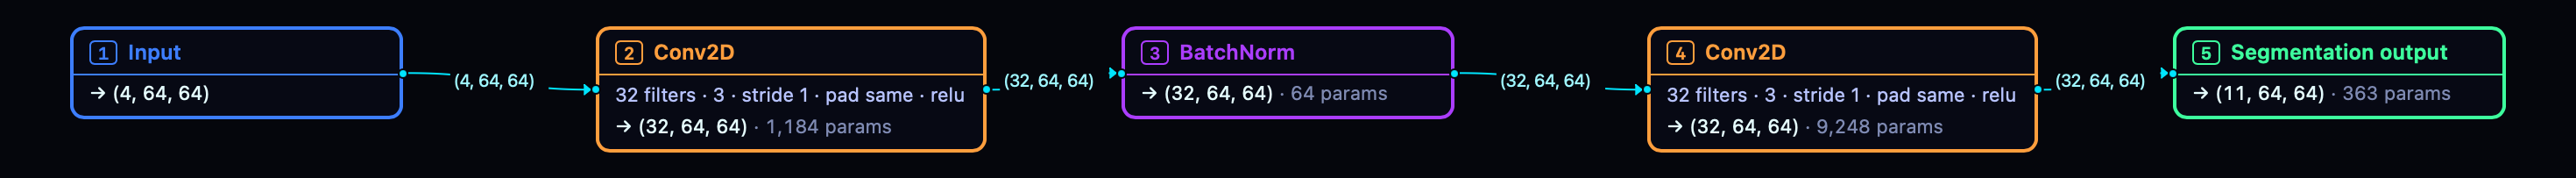
\includegraphics[width=\linewidth,height=0.55\textheight,keepaspectratio]{figures/tests/test19_arch.png}\caption{TEST 19 as a picture: \ui{Save as PNG} on the Design screen (or \ui{File} $\rightarrow$ \ui{Export Design as PNG}) draws the whole design at full size; long designs are split into rows here to fit the page.}\label{fig:test19arch}\end{figure}

The network is small on purpose (1\,184 + 64 + 9\,248 + 363 = 10\,859 parameters): the test is the data path. The Segmentation output has one score per WorldCover class ($32\cdot11+11=363$). After 10 epochs on 48 tiles, built-up land (IoU 0.71) and tree cover (0.67) are learnt; the mean IoU over all 11 classes is only 0.148 because four classes do not occur in the tile and count as 0.

{\small
\begin{longtable}{@{}lp{3.2cm}p{5.4cm}lr@{}}
\toprule
\textbf{Id} & \textbf{Block} & \textbf{Settings} & \textbf{Output} & \textbf{Parameters}\\
\midrule\endhead
t1 & Input & all bands & $4\times64\times64$ & 0\\
t2 & Conv2D & 32 filters, $3\times3$, same, relu & $32\times64\times64$ & 1\,184\\
t3 & BatchNorm &  & $32\times64\times64$ & 64\\
t4 & Conv2D & 32 filters, $3\times3$, same, relu & $32\times64\times64$ & 9\,248\\
t5 & Segmentation output &  & $11\times64\times64$ & 363\\
\midrule
 & \textbf{Total} & & & \textbf{10\,859}\\
\bottomrule
\end{longtable}}
